\documentclass{report}
\usepackage[utf8]{inputenc}
\usepackage[french]{babel}
\usepackage{eurosym}
\usepackage{algorithm}
\usepackage{imakeidx}

\usepackage{algorithmic}
\usepackage{multicol}
\usepackage{graphicx}
\usepackage{xcolor}
\usepackage{tikz}
\usetikzlibrary{trees}
\usepackage{bbold}
\usepackage{lipsum}
\usepackage{amsfonts}
\usepackage{pstricks}
\usepackage{pst-node}
\addtocounter{tocdepth}{3}
\setcounter{secnumdepth}{3}
\usepackage{amsmath}
%pas de numero de chapitre dans les sections
\makeatletter
\renewcommand{\thesection}{\@arabic\c@section}
\makeatother
\newcommand{\E}{\mathbb{E}}

\newcommand{\Var}{\mathbb{V}}


\newcommand{\Cov}{\mathrm{Cov}}
\newcommand{\e}{\mbox{e}}
\newcommand{\dd}{\mathrm{d}}
\newcommand*\markterm[2]{%
	\tikz[remember picture,anchor=base west,baseline,inner sep=0pt, outer sep=0pt]\node(#1){$#2$};%
}
\newcommand{\crule}[3][c]{%
    \par\noindent
    \makebox[\linewidth][#1]{\rule{#2\linewidth}{#3}}}
\newcommand*\arrowtoterm[3][]{%
	\tikz[remember picture,anchor=base west,baseline,inner sep=0pt, outer sep=0pt]\node(x){#3};%
	\tikz[remember picture,overlay,->,shorten <=2pt,shorten >=2pt,#1]\draw(x)to(#2);%
}
\usepackage[mathcal]{euscript}
\usepackage{amssymb}
\usepackage{chronosys}
\setlength{\parindent}{0pt}
\usepackage[left=2cm,right=2cm,top=2.5cm,bottom=2cm]{geometry}
\newcommand{\indep}{\perp \!\!\! \perp}
\usepackage{framed}
\setlength{\FrameSep}{\fboxsep}% séparation entre le texte et le bord
\newcommand{\smallO}[1]{\ensuremath{\mathop{}\mathopen{}o\mathopen{}\left(#1\right)}}
\usepackage{fancyhdr}
\pagestyle{fancy}
\usepackage{ntheorem}
\theoremseparator{. ---}
\newtheorem{prop}{Propri\'et\'e}
\newenvironment{encadre}{%
  \setlength{\theorempreskipamount}{0pt}%
  \setlength{\theorempostskipamount}{0pt}%
  \begin{framed}%
 }{%
  \vspace{-2pt}% ajustement d'espacement en bas
  \end{framed}%
 }

\title{Finance\\Mathématiques Financières\\Actuariat}
\author{}
\date{2021/2022}
\makeindex

\begin{document}

\maketitle
\tableofcontents
\newpage
\chapter{FINANCE}

\section{MARCHES FINANCIERS}
\subsection{principes et utilités des marchés financiers}

Un marché financier\index{Marché!financier} est un lieu de rencontres et d’échanges de produits financiers. Celui -ci est organisé dans le temps (horaires d’ouvertures, etc…)

\noindent%
\begin{minipage}{.5\textwidth}%
\includegraphics[width=8cm]{graph1.png}
\end{minipage}%
\hfill
\begin{minipage}{.55\textwidth}%
Institutions financières : 
\begin{itemize}
    \item Banque de France
    \item Caisse des dépôts 
    \item Banques
    \item OPCDM (organisme de placement de capital en valeur mobilière)
        \begin{itemize}
        \item SICAV (Société d’Investissement à Capital Variable)
        \item FCP (Fond Commun de Placement )
        \end{itemize}
\end{itemize}
\end{minipage}%

Les produits financiers peuvent permettre d’échanger deux choses :
\begin{itemize}
    \item Transfert de capital
    \item Transfert de risques
\end{itemize}

\subsection{Produits financiers}
\subsubsection{Taux d'actualisation et taux d'intérêt}
\index{Taux!d'actualisation}\index{Taux!d'interêt}
Le taux d’intérêt représente la valeur/coût qui permet d’obtenir un capital maintenant. 
Si on considère un produit $F_1$ à la fin de la période (année), sa valeur à l’instant $T_0$ , appelée $F_0$, s’appelle la valeur actualisée de $F_1$ . On a donc $\displaystyle F_0=\frac{F_1}{1+R}$ avec $R$, le taux d’intérêt sur la période.

\subsubsection{Les produits traditionnels}


\begin{description}
    \item [Obligations (Bond) :] l’émetteur est emprunteur / l’acheteur est prêteur.
    Une obligation\index{Obligation}\index{Bond} est un titre de créance (prêt). Elle est caractérisée par trois choses :
    \begin{itemize}
        \item Capital (Emission / Nominal / Rachat)
        \item Taux d’intérêt ( intérêt payé en fin de période/ intérêt payé en fin d’année
        \item Durée
    \end{itemize}

    Il existe plusieurs risques relatifs à ce produit :
    \begin{itemize}
        \item Le risque de défaut ( l’émetteur est susceptible de ne pas payer)
        \item Le risque de taux : « \textit{Quand les taux montent, les prix baissent} »
    \end{itemize}
    \item [Actions (Stock) :]\index{Action}\index{Stock} titre de participation dans une société 
    L’action donne des droits de votes et des droits aux dividendes.
    Il existe les actions ordinaires et les actions de préférence.
    Elle est qualifié par deux choses : la valeur et les dividendes.
    \item [Devises :]
    \item [Matières premières / produits agricoles :] 
\end{description}

\subsubsection{Les produits dérivés}
\index{Produit!dérivé}
\begin{description}
    \item [Les produits dérivés inconditionnels] (contrats à termes => c'est à dire relatif à ce qui va se passer à une date)
    \begin{itemize}
        \item Forwards (moins réglementé)
        \item Futurs (plus règlementé )
        \item Swaps
    \end{itemize}
    Un \textbf{forward}\index{Forward} et un \textbf{futur}\index{Futur} sont des produits qui donnent le droit et l’obligation d’acheter (resp. vendre) un produit sous-jacent à une date donné, et à un prix fixé au départ. 
    
    Les \textbf{futurs} sont réglementés notamment pas les appels de marge. 
    
    Les produits sous-jacents peuvent être un des produits traditionnels ou pas.  
    
    Le \textbf{Swap}\index{Swap} est un contrat d’échange :  on convient qu’à un moment donné, on échangera 2 produits. 
    
    \item [Les produits dérivés conditionnels] (contrats optionnels)
    \begin{itemize}
        \item Options,
        \item Warrants,
        \item Bon de souscription
    \end{itemize}

    Il y a plusieurs types d’\textbf{option} ; par exemple\index{Option} l’option d’achat (resp. de vente)\index{Put}\index{Call} européenne (call, resp. put) : produit qui donne le droit mais pas l’obligation d’acheter (resp.de vendre) un sous-jacent à un prix fixé au début du contrat (prix d’exercice/Strike)\index{Strike} et à une date donné (échéance/horizon)\index{Echéance}\index{Horizon}.
\end{description}

\fbox{%
\begin{minipage}{1\textwidth}
\centering
   \textbf{NB :} \index{Prix !d'exercice}\index{Prix !du sous-jacent}\index{Prix !de l'option}l y a trois prix : le prix de marché du sous-jacent, le prix d’exercice et le prix de l’option
\end{minipage}
}

\fbox{%
\begin{minipage}{1\textwidth}
\centering
   \textbf{REMARQUE :} le prix de marché du sous-jacent est noté $S_t$ à l’instant $T$. Le prix d’exercice est noté $K$, et le prix de l’option est noté $C_T$.
   \centering
   $$
   C_t =
     \left\{
        \begin{array}{ll}
            \ S_t-K & \mbox{si } S_t>K \\
            \ 0 & \mbox{sinon}
        \end{array}
    \right. =\mbox{max}(S_t-K, 0)=(S_t-K)^+
    $$
\end{minipage}
}

\begin{figure}[h!]
    \begin{minipage}[c]{.46\linewidth}
        \centering
        \includegraphics{Image2.png}
        \caption{Prix d’une option d’achat (à T) en fonction du prix du sous-jacent à T}
    \end{minipage}
    \hfill%
    \begin{minipage}[c]{.46\linewidth}
        \centering
        \includegraphics{Image3.png}
        \caption{Prix d’une option de vente (à T) en fonction du prix du sous-jacent à T}
    \end{minipage}
\end{figure}

\vspace{3cm}
"BENEFICE MAX"

\begin{figure}[h!]
    \begin{minipage}[c]{.46\linewidth}
        \centering
        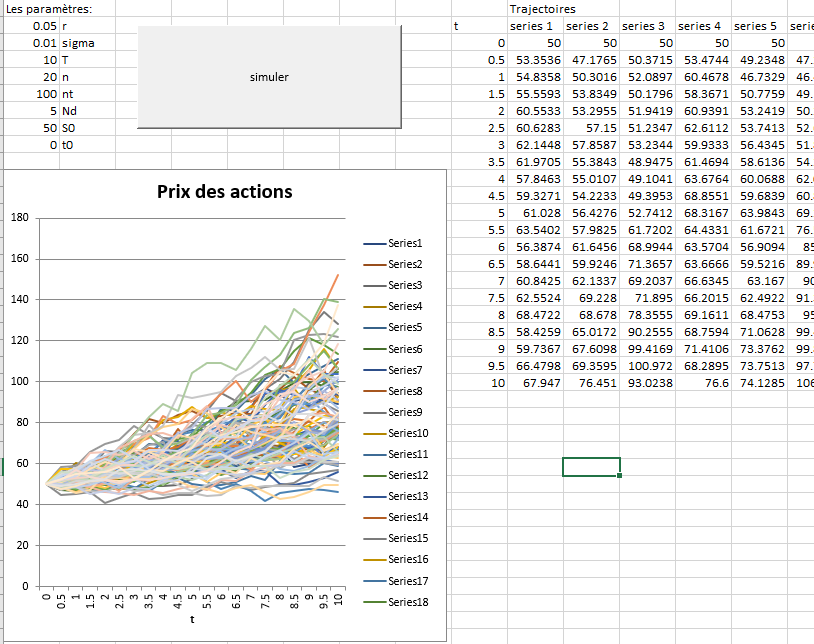
\includegraphics{Capture.PNG}
        \caption{Achat d'une option d'achat}
    \end{minipage}
    \hfill%
    \begin{minipage}[c]{.46\linewidth}
        \centering
        \includegraphics{Capture2.PNG}
        \caption{Vente d'une option de vente}
    \end{minipage}
\end{figure}
\begin{figure}[h!]
    \begin{minipage}[c]{.46\linewidth}
        \centering
        \includegraphics{Capture3.PNG}
        \caption{Achat d'une option de vente}
    \end{minipage}
    \hfill%
    \begin{minipage}[c]{.46\linewidth}
        \centering
        \includegraphics{Capture4.PNG}
        \caption{Vente d'une option de vente}
    \end{minipage}
\end{figure}
\fbox{%
\begin{minipage}{1\textwidth}
\centering
   \textbf{NB :} les ronds bleus indiquent les options de le moins risquée à la plus risquée
\end{minipage}
}
\subsection{Organisation des marchés financiers}

La bourse de Parais a été crée en 1724.

\startchronology[startyear=1980,stopyear=2021]
\chronoevent{1988}{Société de Bourse Française SA (privatisation)}
\chronoevent[markdepth=80pt]{2000}{Euronext : aggrégation de différentes bourses européennes : $ \left\{ \begin{array}{ll} \ \mbox{Paris} \\ \ \mbox{Amsterdam} \\ \ \mbox{Bruxelles} \\ \ \mbox{Lisbonne} \\ \ \mbox{LIFFE = Londres (2002} \end{array} \right.$}
\chronoevent{2007}{NYSE - Euronext}
\chronoevent[markdepth=40pt]{2012}{ICE (Inter Continental Exchange }
\stopchronology

\vspace{2.5cm}
Il existe plusieurs marché :
\begin{enumerate}
    \item \textbf{Marché Primaires}\index{Marché!primaires} : le marché primaire est celui où les sociétés en quête de fonds et les investisseurs se rencontrent pour la première fois. Il s’assimile à une sorte de marché à la criée
    
    Attention, ce marché est différent du premier marché
    \begin{center}
    \LARGE
        $\ne$
    \end{center}
    \textbf{Marchés Secondaires}\index{Marché!secondaire} : On distingue le marché primaire du marché secondaire. Le marché secondaire est celui où s'échangent des titres financiers (ou des objets) d’occasion. Le marché secondaire peut être régulé où mettre directement vendeurs et acheteurs en contact. Il totalise la quasi-totalité des échanges et assure ainsi la liquidité des investissements.
    
    De la même manière, il est différent du second marché
    
    
    \item \textbf{Marchés règlementés/ organisés/ gré à gré :} 
    
    \begin{center}
    premier marché\index{Premier Marché} / second marché\index{Second marché} / nouveau marché\index{Nouveau marché}
    
    $\Longrightarrow$
    
    de plus en plus risqué
    \end{center}
\end{enumerate}

\subsection{Fonctionnement du marché boursier\index{Marché!boursier}}

Le marché boursier est le lieu de rencontre entre l'offre et la demande.

\begin{description}
    \item [CAC 40 :\index{CAC 40}] indice qui est fait sur unr un portefeuille constituée des 40 actions françaises les plus puissantes. (Cotation assisté en continue)
\end{description}

Il y a 2 types de cotations : 
\begin{itemize}
    \item en continue\index{Cotation!en continue} (toutes heures du jour mais pas de nuit - 9h 17h en France -)
    \item au fixing\index{Cotation!au fixing} (valorisation quotidienne ou biquotidienne)
\end{itemize}

La \index{Cours!de l'action}cours de l'action est le montant de la dernière transaction

il y a un \index{carnet d'ordres}carnet d'ordres : 

\begin{figure}[h!]
       \centering
        \includegraphics[width = 8cm]{feuille_de_marche.PNG}
        \caption{Carnet d'ordre de Lagardère}
\end{figure}

\hspace{1cm}

\subsection{Analyse d'un obligation à taux fixe}

\subsubsection{Rappel sur les taux d'interêt\index{Taux!d'interêt}}
On emprunte un capital $C$ au taux $R$ sur une periode (\textit{e.g.} 1 an).

On rembourse à la fin de la période $\displaystyle C+C\times R = C(1+R)$

Sur $n$ périodes : \begin{itemize}
    \item \textbf{Taux proportionnel\index{Taux!proportionnel} :} 
    \begin{center}
        $C(1+R)^n$
    \end{center}
    Les interêts ne sont pas capitalisés
    \vspace{0.3cm}
    \item \textbf{Taux d'interêt composé\index{Taux!d'interêt composé} :} 
    
\hspace{1cm}
    Les interêts sont capitalisés : ils sont ajoutés au capital, et produisent à leurs tours des interêts
\end{itemize}

\vspace{0.7 cm}
On peut déterminer un taux d'interêt pour une sous période : 

\hspace{1cm}
On suppose qu'il y a $k$ sous période dans 1 période (\textit{e.g.} $k=12$, sous période = 1 mois)

\hspace{1cm}
On note $R_k$ le taux de sous période

\hspace{1cm}
On peut avoir un \textbf{taux proportionnel} ou un\textbf{ taux actuariel/taux équivalent : }
\hspace{1cm}
\begin{itemize}
    \item \textbf{Taux proportionnel :}
    \begin{center}
        $\displaystyle R_k=\frac{R}{k}$
    \end{center}
    \item \textbf{Taux actuariel/équivalent :}
    \begin{center}
        $\displaystyle \mbox{On cherche } R_k \mbox{ tq. } (1+R_k)^k = 1+R$
    \end{center}
    (cela suppose que les intérêts sont capitalisés en fin de sous période)
\end{itemize}

\fbox{%
\begin{minipage}{1\textwidth}

   \textbf{REMARQUE 1:} Si $t$ correspond à un nombre entier de sous période (18 mois, 1.5 an = 1.5 sous période)
  \begin{center}
      $t=p$ sous période $=\displaystyle\frac{p}{k}$ période
   
   $C\rightarrow C(1+R_k)^p=C(1+R_k)^{tk}=C(1+R)^t$
  \end{center} 
   
   
   Ainsi la formule $C\rightarrow C(1+R)^n$ vue pour n périodes reste valable pour un nombre non entier de périodes (par ex. 1.5) mais de la forme $\displaystyle t=\frac{n}{k}$ or $k^$ est ici arbitraire donc on peut prendre $k$ très grand de sorte que la fromule est valable pour $k\in \mathbb{Q}$ et par continuité pour $t \in \mathbb{R}$
\end{minipage}
}

\fbox{%
\begin{minipage}{1\textwidth}

   \textbf{REMARQUE 2:} on peut écrire $(1+R)^t$ sous la forme $\mbox{e}^{t \mbox{ln}(1+R)}$
   
   Si on pose $r = \mbox{ln}(1+R)$, on a $(1+R)^t=\mbox{e}^{rt} \Longrightarrow\mbox{e}^r = 1+R $ 
   
   Avec ces notations \centering \fbox{$\displaystyle C\rightarrow_t C\mbox{e}^{rt}$}
\end{minipage}
}

\fbox{%
\begin{minipage}{1\textwidth}

   \textbf{REMARQUE 3:}Ne pas confondre la remarque 2 avec celle-ci : 
   
   Si on considère un taux de période $R$, et que l'on calcule le taux d'une sous période auto-proportionnel $\displaystyle R_k = \frac{R}{k}$
   
  \fbox{ET} que l'on capitalise le sintérêts en fin de sous période, alors à la fin de la période
  \begin{center}
      $C\rightarrow_t C(1+\frac{R}{k})^k$
  \end{center}
  
  Si de plus, $_ \rightarrow \infty$
  
  
 \begin{center}
  $\displaystyle\lim_{k \rightarrow \infty} (1 + \frac{R}{k})^k = \lim_{k \rightarrow \infty} \mbox{e}^{\displaystyle k\mbox{ln}(1+\displaystyle\frac{R}{k})}$
  
  or $\mbox{ln}((1+\displaystyle\frac{R}{k}) = \frac{R}{k}(1+\varepsilon_k) \mbox{ avec } \displaystyle\varepsilon_K\rightarrow 0$
  
  $k\mbox{ln}(1+\displaystyle\frac{R}{k})=R(1+\varepsilon_k)\rightarrow_{k \to \infty} R$\footnote{$\mbox{ln}(1+x)=x+x\times \varepsilon_x$}
  \end{center}
  
De plus,
\centering
 .....
\end{minipage}
}

\subsubsection{Taux d'actualisation}

Un flux à un instant $t$ n'a pas la même valeur que ce même flux à l'instant $0$.

La valeur à $t=0$ du flux $F_t$ est $\displaystyle\frac{F_t}{(1+R)^t}$

$\tilde{F_t} = \displaystyle\frac{F_t}{(1+R)^t}$ est le taux actualisé du flux $F_t$

$R$ est le taux supposé constant sur la période $[0;t]$

On peut généraliser le concept : par exemple si $t=n \in \mathbb{N}$ et si $R_1,R_2,\mbox{...,}R_n$ sont les taux annuels pour les périodes $[0;1]$,$[1;2]$

Plus généralement encore, si on considère 1 ensemble de flux $F_t_1...F_t_n$ aux temps $t_1...t_n$ la valeur actualisé de cet ensemble est la somme algébrique $\displaystyle\sum^n_{i=1}\frac{F_t_i}{(1+R)^{t_i}} = \displaystyle\sum^n_{i=1} \mbox{e}^{-rt_i}F_t_i$ avec $r = \mbox{ln}(1+R)$

\subsubsection{Dynamique d'une obligation zero coupon}

Si on note $P_t$, la valeur de l'obligation à l'instant $t$

On voit que $P_t = P_0\ \mbox{e}^{rt}=P_0(1+R)^t$

On a alors $\displaystyle\frac{\mathrm{d}P_t}{\mathrm{d}t} =   P_0\ \mbox{e}^{rt} = rP_t \Rightarrow \displaystyle\frac{\mathrm{d}P_t}{P_t} = r\mathrm{d}t$\footnote{$y = f(x) \Rightarrow \displaystyle \frac{\mathrm{d}y}{\mathrm{d}x} = f'(x) \Rightarrow \mathrm{d}y = f'(x)\mathrm{d}x$}


\fbox{%
\begin{minipage}{1\textwidth}

   \textbf{REMARQUE :} si $P_t$ verifie $\displaystyle\frac{\mathrm{d}P_t}{P_t} = r\mathrm{d}t$
   
   Alors comme $\displaystyle\frac{\mathrm{d}P_t}{P_t} = \mathrm{d}(\ln(P_t))$
   
   On a 
   \centering
   $\mathrm{d}(\ln(P_t)) = r\mathrm{d}t$
   
   $\underbrace{\displaystyle\int^t_0\mathrm{d}(\ln(P_t))}_{\displaystyle\ln(P_t)-ln(P_0) = \displaystyle\ln\left(\frac{P_t}{P_0}\right)} = \displaystyle\int^t_0r\mathrm{d}t = r\times t $
   
   $\Rightarrow P_t = P_0\mbox{e}^{rt}$
   
\end{minipage}
}

\subsection{Analyse d'une action}
\subsubsection{Etude de la dynamique}
On note $P_t$, le prix de l'action à l'instant $t$.
\begin{center}
    $\displaystyle\frac{P_{t+\Delta t} - P_t}{P_t}$ = evolution $\approx \beta \Delta t = \mbox{ rendement moyen}$
\end{center}

On suppose que $\displaystyle\frac{P_{t+\Delta t} - P_t}{P_t} \approx \beta_{\Delta t} + Z_{t,t+\Delta t}$ avec $Z_{t,t+\Delta t} \sim \mathcal{N}(m,\,\sigma)$

On suppose que le prix est à "accroissements indépendants"

Soit trois temps $t, t' \mbox{ et } t''$ : $P_{t''}-P_{t'} \indep P_{t'}-P_t \Rightarrow \displaystyle\frac{P_{t''}-P_{t'}}{P_{t'}} \indep \displaystyle\frac{P_{t'}-P_t}{P_t}$, car on neglige la variation entre $t$ et $t'$.

On a $Z_{t,t'} \indep Z_{t',t''}$ et $Z_{t,t''} \approx Z_{t,t'}+Z_{t',t''} \Rightarrow \mathbb{V}(Z_{t,t''}) = \mathbb{V}(Z_{t,t'})+\mathbb{V}(Z_{t',t''})$\newline
On suppose que le modèle est stationnaire \textit{i.e.} $\mathbb{V}(Z_{t,t'})=h(t'-t)$\newline
On doit avoir 
\begin{eqnarray}
h(t''-t) & = & h(t''-t'+t'-t) \nonumber\\
& = & h(t''-t')+h(t'-t) \nonumber
\end{eqnarray}
En d'autres termes : 
\begin{eqnarray}
h(u+v) & = & h(u)+h(v)\Rightarrow h(u) = u\ h(1) \nonumber\\
\mathbb{V}(Z_{t,t'})& = & (t'-t)\ \underbrace{h(1)}_{\mbox{cst}}= (t'-t)\ c \nonumber
\end{eqnarray}
\begin{center}
    $Z_{t,t'} \sim \mathcal{N}(0,\sigma \sqrt{t'-t})\mbox{ avec } \sigma = \sqrt{c}$
\end{center}

\vspace{0.5cm}
Il existe un processus noté $\left(W_t\right)_t$ qui verifie







\setlength{\columnsep}{100pt}
$\mbox{\fbox{MOUVEMENT BROWNIEN}}
\left\{ \hspace{2cm}\begin{array}{ll} 
-W_0 = 0 \mbox{ et } W_t \mbox{ est } \EuScript{F}_t\mbox{-mesurable}\\ 
-t\to W_t \mbox{est continu pour presque tout }\omega \in \Omega \\ 
-W_{t'}-W_t \sim \mathcal{N}(0, \sqrt{t'_t)})\\
-W_{t'}-W_t \indep \EuScript{F}_t \footnotemark
\end{array} \right.$
\footnotetext{$\EuScript{F}_t$ : tout ce qui est connu  jusqu'à $t$}

\vspace{0.5cm}
Ainsi, $Z_{t,t'} = \sigma(W_{t'}-W_t)$\footnote{$X\sim\mathbb{N}(0,\sigma)$\hspace{0.5cm}\\$X=\sigma N\Rightarrow N\sim \mathbb{N}(0,1)$}, et donc $\displaystyle\frac{P_{t+\Delta t} - P_t}{P_t} = \beta_{\Delta t} + \sigma (W_{t+\Delta t}-W_t)$\\
Et quand les accroissements sont infiniments petits
\begin{eqnarray}
\displaystyle\frac{P_{t+\mathrm{d} t} - P_t}{P_t} & = & \beta\mathrm{d} t+ \sigma \underbrace{(W_{t+\mathrm{d} t}-W_t)}_{\mathrm{d}W_t} \nonumber\\
& = & \underbrace{\beta\mathrm{d} t+ \sigma \mathrm{d}W_t\footnotemark}_{\mbox{MODELE DE BLACK-SHOLES}} \nonumber
\end{eqnarray}
\footnotetext{EDS : Equation differentielle stochastique}

\subsection{Portefeuille Autofinancé}
On considère un portefeuille constitué de $n+1$ actifs de prix $p_0^t\dots p^n_t$.
\begin{itemize}
    \item $p^0 = $ actif "sans risque" $\Rightarrow$ obligation
    \item $p^1_t\to p^n_t = $ des biens risqués" $\Rightarrow$ actions
\end{itemize}
Les actifs sont détenus dans les quantités $Q_t^0\dots Q^n_t$. Les quantités evoluent à certains instants $t_0\dots t_n$.

on note $V_t$ la valeur du portefueille : $V_t = \displaystyle\sum_0^n Q_t^iP_t^i$
\begin{eqnarray}
V_{t_{i+1}}-V_{t_i} & = & \displaystyle\sum_0^n Q^k_{t_{i+1}}P^k_{t_{i+1}} \nonumber \\
V_{t_{i+1}}-V_{t^-_{i+1}}+V_{t^-_{i+1}}-V_{t_i} & = & \displaystyle\sum_0^n P^k_{t_{i+1}}\left(Q^k_{t_{i+1}}-Q^kk_{t^-_{i+1}}\right) + \displaystyle\sum_0^n Q^k_{t_{i}}\left(P^k_{t_{i+1}}-P^k_{t_i}\right)\nonumber
\end{eqnarray}
On pose $\Delta X_{t_i} = X_{t_{i+1}}-X_{t_i} \Rightarrow \Delta V_{t_i} = \displaystyle\sum_0^n P^k_{t_{i+1}}\Delta Q^k_{t_i} + \displaystyle\sum_0^n Q^k_{t_{i}}\Delta P^k_{t_{i}}$

Le portefeuille est \textbf{autofinancé} si $\displaystyle\sum_0^n P^k_{t_{i+1}}\Delta Q^k_{t_i} = 0$, autrement dit si $V_{t_{i+1}}-V_{t^-_{i+1}} = 0, \forall i$\\
Donc dans le cas d'un portefeuille autofinancé, il reste 
\begin{center}
    $\Delta V_{t_i} = \displaystyle\sum_0^n Q^k_{t_{i}}\Delta P^k_{t_{i}}$
\end{center}
Si $\sup(t_{i+1}\to 0 \Rightarrow \Delta V_{t_i} \to \mathrm{d}V_{t_i}$
\begin{center}
    $\mathrm{d} V_{t_i} = \displaystyle\sum_0^n Q^k_{t_{i}}\mathrm{d} P^k_{t_{i}}$
\end{center}

\vspace{3cm}
\section{Limie de la valorisation en espérance - AOA}
\subsection{Valorisation d'un jeu de pile ou face}
On considère plusieurs contrats : si c'est pile je gagne $X$ \euro, sinon je gagne 0 \euro.\\
\textit{Par exemple, à quel prix j'acheterais un ticket si j'ai $1/2$ de gagner 200 \euro}\\
Plus les sommes sont élévées, plus les pertes possibles sont élevées. \\

\subsection{Paradoxe de Saint Petersbourg}
On gagne 2 \euro si on tombe sur pile pour la première fois au $n^{ieme}$ coup.
\begin{eqnarray}
\mathbb{E}(G)&=& 2\times \frac{1}{2}+4\times \frac{1}{4}+\dots+2^k\times \frac{1}{2^k}+\dots \nonumber\\
&=& \mathbb{E}(2^X) \mbox{      avec $X$ : instant aléatoire où l'on gagne}\nonumber \\
&=& \displaystyle\sum_k 2^k\mathbb{P}(X=k) = +\infty\nonumber 
\end{eqnarray}
L'éspérence de gain est infini mais ca n'aurait pas de sens de valoriser ce contrat à l'infini.\\
On a aussi \begin{eqnarray}
\mathbb{P}(X\geq n_0)&=& \displaystyle\sum_{k=4}^\infty \frac{1}{2^k}\nonumber \\
&=& \frac{1}{2^{n_0}}(1+\frac{1}{2}+\frac{1}{4}+\dots)\nonumber\\
&=& \frac{1}{2^{n_0}}\left(\frac{1}{1-\frac{1}{2}}\right)\nonumber\\
&=&\frac{1}{2^{n_0-1}}\nonumber
\end{eqnarray}
Par exemple, si on mise 8 \euro on a 7 chance sur 8 de perdre.

\subsection{Fonction d'utilité}
\noindent%
\begin{minipage}{.5\textwidth}%
\includegraphics[width=8cm]{utilite.PNG}
\end{minipage}%
\hfill
\begin{minipage}{.55\textwidth}%
La courbe d'utilité est une fonction concave\footnotemark et croissante. \\
Ce shéma correspond à la situation où la valeur du contrat coïncide avec l'espérance des gains\\
\textit{"Le jeu n'en vaut pas la chandelle"}; en effet on voit que $|u(F_0)-u(F_0-h)|>|u(F_0)-u(F_0+h)|$ avec $\mathbb{P}(F_0+h)=1/2$ et $\mathbb{P}(F_0-h)=1/2$
\end{minipage}%
\footnotetext{sous sa tante est $f''<0 \Leftarrow u(a+h)-u(a)>u(b+h)-u(b) \mbox{ pour } a<b$}
Pour équilibrer le risque, on peut mettre un prime de risque. Par exemple, en termes d'utilité, perdre 400 \euro pourrait revenir à gagner 600 \euro.

\vspace{0.2cm}
Le calcul de l'espérance n'est pas une bonne valorisation.\\
Il y a deux cas ou la valorisation pas l'espérance est pertinent :
\begin{itemize}
    \item quand la loi des grands nombre s'applique
    \item quand la fonction d'utilité est linéaire
\end{itemize}

\begin{center}
    Dans le cas ou la fonction est concave, l'acteur est averse aux risques
    
    Dans le cas où la fonction est convexe, l'acteur a le goût du risques.
\end{center}

\subsection{Valorisation d'un contrat Forward (contrat à terme)}
\fbox{
\begin{minipage}{1\textwidth}
\begin{description}
    \item [Opportunité d'arbitrage : ] Il y a une opprotunité d'arbitrage chaque fois qu'une transaction assure un profit certain sans dépense initale. Autrement sit, il existe une situation d'arbitrage lorsqu'il est possible de réaliser un profit sans risque et sans apport de fonds par combinaison de deux ou plusieurs transactions. 
    \begin{description}
        \item [\textit{exemple : }] $\ $\\
        Une action est cotée dans deux bourses différentes. Il suffit d'acheter au prix le plus bas et vendre simultanément au prix le plus haut.\\
        Le profit est immédiat et sans risque.\\
        Cette situation ne peut pas durer dans un marché éfficient.\\
        L'afflut des ordres d'achat va faire monter le prix et l'afflux des ordres de ventes va le faire baisser, jusqu'à légalité des prix (équilibre du marché). D'où la disparition de l'opportunité d'arbitrage.
    \end{description}
\end{description}
\end{minipage}
}

\vspace{0.2cm}
Soit un contrat à terme sur une action de prix $(S_t)_t$, avec un prix d'exercice $K$. On suppose que le taux d'intérêt instantané du marché est $r$. La valeur du froward à $t=0$ est nulle.\\
On peut emprunter au taux $r$ une somme $C\to C \mbox{e}^{rT}$ à l'instant $T$.
\[ C \mbox{e}^{rT} = C(1+R)^T \mbox{ avec } r = \ln(1+R)^T\]

\vspace{0.2cm}
Valoriser le contrat revient à déterminer $K$. \\
A terme l'acheteur du forward encaisse $S_t-K$ si $S_t-K$ est positif, et paye $K-S_t$ sinon.

\vspace{0.3cm}
\underline{Quelle est la valeur correcte de K ?}\\
$S_0$, $r$ et $T$ sont connus\\
On pourrait être tenter d'utiliser comme prix d'exercice a terme, l'espérance du prix $S_t$. Mais il existe une autre stratégie qui impose une valeur au prix d'exercice : c'est le principe d'\textbf{absence d'opportunité d'arbitrage}.\\
Dans le cas présent on va montrer que \[K=S_0\mbox{e}^{rT}\]


\begin{description}
    \item [Démo : ] $\ $
    \begin{itemize}
        \item Supposons $K>S_0\mbox{e}^{rT}$\\
        On peut "vendre"\footnote{il n'y a pas de transfert d'argent à ce moment là} le forward et on achète le sous-jacent $S_0$ à $t=0$ en empruntant au taux $r$.\\
        A terme, on rembourse $S_o\mbox{e}^{rT}$ en vendant comme convenu le sous-jacent au prix d'exercice K. On conserve ainsi $K-S_o\mbox{e}^{rT}>0$.\\
        On peut bénéficier de la somme $\mbox{e}^{-rT}(K-S_o\mbox{e}^{rT})$ dès l'instant $0$ en empruntant cette somme que l'on remboursera à $T \to \mbox{e}^{rT}(\mbox{e}^{-rT}(K-S_o\mbox{e}^{rT})) = K-S_o\mbox{e}^{rT}$\\
        Cette situation ne peut pas exister durablement.
        \item Supposons maintenant que $K<S_0\mbox{e}^{rT}$\\
        Les détenteurs de l'action peuvent bénéficier d'une opportunité d'arbitrage.\\
        Ils vendent l'action au prix $S_0$, ils placent le montant au taux $r$, et ils "achètent"\footnote{il n'y a pas de transfert d'argent} le forward.\\
        A terme, ils achètent l'action au prix $K$ et ils touchent le montant du placement avec les interêts $S_0\mbox{e}^{rT}$.\\
        Au bilan, il ont gagné $S_0\mbox{e}^{rT}-k$ et ils ont de nouveau l'action.
    \end{itemize}
    Dans un marché à l'équilibre, il n'y a pas d'opportunité d'arbitrage. 
\end{description}
 







\section{Valorisation d'une option}
\subsection{Modèle Binomiale à 1 période}

On considère une action au prix $S_t$ avec $t = \{0,1\}$ et une option (achat ou vente) de prix $C_t$ et de prix d'exercice $K$.\\
On suppose que l'on peut acheter ou vendre des obligations au taux $r$.\\
\begin{multicols}{2}
$\ $\\$\ $\\$\ $
On suppose que l'on a 2 possibilité à $t=1$ : ($S_1^b<S_1^h$)

\begin{tikzpicture}
    \tikzstyle{level 1}=[level distance=4cm, sibling distance=2cm]
    \node{$S_0$}[grow=right]
    child{node{$S_1^b$}
      edge from parent node[below]{$P_b$}}
    child{node{$S_1^h$}
      edge from parent node[above]{$P_h$}};
\end{tikzpicture}

\end{multicols}
On cherche $C_0$, on commence donc par observer $C_1$ qui prend soit la valeur $C_1^h$ soit $C_1^b$. Par exemple, si on a une option d'achat $C_1(S_1) = (S_1-K)^+$\\
Pour trouver $C_0$, on constitue un portefeuille constitué d'actions et d'obligations de façon à dupliquer le prix de l'option à $t=1$.\\
On veut avoir $V_1\equiv C_1 \Leftrightarrow \left\{\begin{array}
     V_1^h = C_1^h \\
     V_1^b = C_1^b
\end{array}\right.$
Le portefeuille contient $x$ actions et $y$ obligations de prox $B_t$ de sorte que $V_t = xS_t+yB_t$\\
On doit avoir $\left\{\begin{array}
     xS_1^h+yB_1=C_1^h \\
     xS_1^b+yB_1=C_1^b
\end{array}\right.\Righarrow \left\{\begin{array}{r}
     \ x = \displaystyle\frac{C_1^h-C_1^b}{S_1^h-S_1^b}  \\
     y = \displaystyle\frac{C1^hS_1^b-C_1^bS_1^h}{B_1(S_1^b-S_1^h)}
\end{array}\right.$
Ce portefeuille duplique le prix de l'option à l'instant terminal $\Righarrow $ c'est un portefeuille de couverture.\\


\begin{minipage}{0.65\textwidth}%
L'absence d'opportunité d'arbitrage implique \begin{eqnarray}
C_0&=&V_0\nonumber\\
&=& xS_0+yB_0\nonumber\\
&=&\displaystyle\frac{C_1^h-C_1^b}{S_1^h-S_1^b}S_0+\displaystyle\frac{C_1^hS_1^b-C_1^bS_1^h}{B_1(S_1^b-S_1^h)}B_0\nonumber \\
&=&\displaystyle\frac{C_1^h-C_1^b}{\mu^h-\mu^b}+\displaystyle\frac{1}{1+R}\displaystyle\frac{C_1^h(1+\mu^b)-C_1^b(1+\mu^h)}{\mu^h-\mu^b}\nonumber \\
&=& C_1^h\displaystyle\frac{1+R-(1+\mu^b)}{(\mu^h-\mu^b)(1+R)}+C_1^b\displaystyle\frac{(1+\mu^h)-(1+R)}{(\mu^h-\mu^b)(1+R)}\nonumber\\
&=&\displaystyle\frac{1}{1+R}\left[C_1^h\displaystyle\frac{R-\mu^b}{\mu^h-\mu^b}+C_1^b\displaystyle\frac{\mu^h-R}{\mu^h-\mu^b}\right]\nonumber
\end{eqnarray}
\end{minipage}%
\hfill
\fbox{
\begin{minipage}{0.35\textwidth}%
On pose $\displaystyle\frac{S_1^h}{S_0}=1+\mu^h$ et $\displaystyle\frac{S_1^b}{S_0}=1+\mu^b$ avec $\mu=$ rendement\\ et $\displaystyle\frac{B_1}{B_0}=1+R$
\end{minipage}%
}
On pose $\Pi^h = \displaystyle\frac{R-\mu^b}{\mu^h-\mu^b}$ et $\Pi^b = \displaystyle\frac{\mu^h-R}{\mu^h-\mu^b}$\\
On a $Pi^b>0$ et $\Pi^h>0$ et $¨\Pi^b+\Pi^h=1$\\
donc \[C_0=\displaystyle\frac{1}{1+R}\left[C_1^h\Pi^h+C_1^b\Pi^b\right]\]
Si on note $\Pi$\footnote{probabilité risque neutre} la proba $(\Pi^h,\Pi^b)$ sur l'univers $\{b,h\}$, alors \[C_0=\displaystyle\frac{1}{1+R}\mathbb{E}_\Pi(C_1)\]
On a $\tilde{C_1}\footnotemark=\displaystyle\frac{C_1}{1+R}$
\footnotetext{Valeur actualisée à $t=0$ de $C_1$}
Ainsi \[\fbox{\tilde{C_0}=C_0=\mathbb{E}_\Pi(\tilde{C_1})}\]
\begin{center}
    \textbf{NB : }on peut utiliser l'espérance car c'est un risque neutre (fonction d'utilité linéaire)
\end{center}

\fbox{
\begin{minipage}{1\textwidth}
\begin{description}
    \item [Probabilité risque neutre : ] c'est la probabilité vrtuelle pour laquelle tous les processus actualisés sont des martingales. 
\end{description}
\end{minipage}
}

On a aussi \begin{eqnarray}
\mathbb{E}_\Pi(\tilde{S_1})&=&\mathbb{E}_\Pi(\displaystyle\frac{S_1}{R+1})\nonumber\\
&=&\displaystyle\frac{1}{1+R}\left[S_1^h\displaystyle\frac{R-\mu^b}{\mu^h-\mu^b}+S_1^b\displaystyle\frac{R-\mu^h}{\mu^h-\mu^b}\right]\nonumber\\
&=&\displaystyle\frac{S_0}{1+R}\left[(1+\mu^h)\displaystyle\frac{R-\mu^b}{\mu^h-\mu^b}+(1+\mu^b)\displaystyle\frac{R-\mu^h}{\mu^h-\mu^b}\right]\nonumber\\
&=&S_0\nonumber
\end{eqnarray}


\subsection{Modèle binomiale à $n$ périodes}
On considère une action sur n périodes et on suppose qye les possibilités constituent un arbre binomial recombinant 
$$\left.\begin{array}{cc}
\begin{tikzpicture}
    \tikzstyle{level 1}=[level distance=3cm, sibling distance=2cm]
    \tikzstyle{level 2}=[level distance=3cm, sibling distance=2cm]
    \node{}[grow=right]
    child{node{}
      child{node{}           edge from parent node[below]{$P^b^b$}}
      child{node{}           edge from parent node[below]{$P^b^h$}}
      edge from parent node[below]{$P^b$}}
    child{node{}
      child{node{}           edge from parent node[below]{$P^h^b$}}
      child{node{} edge from parent node[below]{$P^h^h$}}
      edge from parent node[below]{$P^h$}};
\end{tikzpicture}\end{array}\right\}...\ (n+1) \mbox{ possibilités au rang }n
$$

Le prix terminal $C_n$ est connu de façon récursive.\\
On peut calculer le prix partout.Pour cela, on fait apparaitre une proba $\Pi$  sur l'univers $\{h,b\} = \{(x_1,\dots, x_n), x_i\in \{h,b\} $ 
\begin{center}
    $C_n = \mathbb{E}_\Pi\left[ \displaystyle\frac{C_{n+1}}{(1+R)^n} / \EuScript{F}_n\right]$\\
    $\frac{C_n}{(1+R)^n} = \mathbb{E}_\Pi\left[ \displaystyle\frac{C_{n+1}}{(1+R)^{n-1}} / \EuScript{F}_n\right]$\\
    $\underbrace{\tilde{C}_n = \mathbb{E}_\Pi\left[ \tilde{C_{n+1}} / \EuScript{F}_n\right]}_{\mbox{Martingale}}$
\end{center}

Ainsi, $\tilde{C}_n$ et un martingale sur $\Pi$.\\
On observe que la proba risque neutre ne dépend que des rendements $\mu^b, \mu^h$ ete $R$ pourchaque "gnomon".
\begin{multicols}{2}
\centering
$\Pi^h = \displaystyle\frac{R-\mu^b}{\mu^h-\mu^b}$\\
$\Pi^b = \displaystyle\frac{\mu^h-R}{\mu^h-\mu^b}$
\end{multicols}
Le prix terminla de l'option n'intervient pas. Seuls interviennent les valeurs du sous-jacent.\\
Par conséquent, la proba $\Pi$ est la même quelque soit l'option valorisée.



\subsection{Formule de valorisation en temps continu}
On se place dans le modèle de BLACK-SCHOLES, et on considère une action de prix $S_t$ et une obligation de prix $B_t$ ($t\in [0,T]$).
On a $\displaystyle\frac{\mathbf{d}S_t}{S_t} = \underbrace{\beta\mathrm{d}t+\sigma\mathrm{d}W_t}_{\mbox{On fluctue autour du rendement moyen}}$ et $\displaystyle\frac{\mathrm{d}B_t}{B_t}=r\mathrm{d}t$\\
et on considère une option sur le sous-jacent $S_t$, de prix d'exercice $K$ au terme $T$ et de prix $C_t$.\\
Onn considère un portefeuille constitué d'actions et d'obligations de valeur $V_t$. On note $\psi_T$ et $\varphi_T$ les quantités d'actions et d'obligations : \[V_t = \psi_tS_t+\varphi_tB_t\]\\
On suppose que le portefeuille est autofinancé donc \[\mathrm{d}V_t = \psi_t\mathrm{d}S_t+\varphi_t\mathrm{d}B_t\]
\begin{eqnarray}
\tilde{V}_t&=& \mbox{e}^{-rt}V_t\nonumber\\
\mathrm{d}\tilde{V}_t &=& -r\mbox{e}^{-rt}[\psi_tS_t+\varphi_tB_t\mathrm{d}t]+\mbox{e}^{-rt}\mathrm{d}V_t\nonumber\\
&=& -r\mbox{e}^{-rt}V_t\mathrm{d}t+\mbox{e}^{-rt}[\psi_t\mathrm{d}S_t+\varphi_t\mathrm{d}B_t]\nonumber\\
&=& \psi_t\underbrace{\left[-r\mbox{e}^{-rt}S_t\mathrm{d}t+\mbox{e}^{-rt}\mathrm{d}S_t\right]}_{\mathrm{d}(\underbrace{\mbox{e}^{-rt}S_t}_{\tilde{S}_t})}+\varphi_t\underbrace{\left[-r\mbox{e}^{-rt}B_t\mathrm{d}t+\mbox{e}^{-rt}\mathrm{d}B_t\right]}_{\mathrm{d}(\mbox{e}^{-rt}B_t)\footnotemark=\mathrm{d}B_0=0}\nonumber\\
\mathrm{d}\tilde{V}_t&=&\psi \mathrm{d}\tilde{S}_t\nonumber
\end{eqnarray}
\footnotetext{$\frac{\mathrm{d}B_t}{B_t}=r\mathrm{d}t\Righarrow B_t = B_0\mbox{e}^{rt}\Righarrow \mbox{e}^{-rt}B_t=B_0$}


\fbox{
\begin{minipage}{1\textwidth}
\begin{description}
    \item [Théorème de Girsanov : ]\textit{"Modifier les probas des trajectoires possibles pour obtenir un brownien"}\\
    On considère une mouvement brownien $(W_t)_t$.\\
    On pose $W't = W_t+\displaystyle\frac{\beta-r}{\sigma}t$\\
    $W'$ n'est pas un mouvement brownien pour la proba $P$ (proba réelle). Mais il existe une probabilité $\Pi$ sur l'ensemble des trajectoires pour laquelle $(W'_t)_t$ est un mouvement brownien.
    
    \fbox{%
\begin{minipage}{0.7\textwidth}
\centering
   \textbf{NB :} Pour la proba $\Pi$, $W_t$ n'ets pas un mouvement brownien
\end{minipage}
}
\end{description}
\end{minipage}
}


\subsection{APPLICATION}
On a $\displaystyle\frac{\mathbf{d}S_t}{S_t} = \beta\mathrm{d}t+\sigma\mathrm{d}W_t$ 

\begin{eqnarray}
\tilde{S}_t = \mbox{e}^{-rt}S_t \Righarrow \mathrm{d}\tilde{S}_t&=&-\mbox{e}^{-rt}S_t\mathrm{d}t+\mbox{e}^{-rt}\mathrm{d}S_t\nonumber\\
&=&-r\tilde{S}_t\mathrm{d}t+\mbox{e}^{-rt}\left[S_t\beta \mathrm{d}t+S_t\sigma\mathrm{d}W_t\right]\nonumber\\
&=&-r\tilde{S}_t\mathrm{d}t+\tilde{S}_t\beta\mathrm{d}t+\tilde{S}_t\sigma\mathrm{d}W_t\nonumber\\
&=&\tilde{S}_t\left[-r\mathrm{d}t+\beta\mathrm{d}t+\sigma\mathrm{d}W_t\right]\nonumber\\
&\Righarrow&\displaystyle\frac{\mathrm{d}\tilde{S}t}{\tilde{S}_t} = (\beta - r)\mathrm{d}t+\sigma\mathrm{d}W_t\nonumber
\end{eqnarray}
on a alors, avec $W'_t$, un mouvement broxnien pour la proba risque neutre $\Pi$ : 
\begin{eqnarray}
\displaystyle\frac{\mathrm{d}\tilde{S}t}{\tilde{S}_t} &=& (\beta - r)\mathrm{d}t+\sigma\left[\mathrm{d}W'_t-\displaystyle\frac{\beta-r}{\sigma}\mathrm{d}t\right]\nonumber\\
&=&\sigma \mathrm{d}W'_t \nonumber\\
\mathrm{d}\tilde{S}_t&=&\tilde{S}_t\sigma \mathrm{d}W'_t \nonumber
\end{eqnarray}
Or on sait que $\mathrm{d}\tilde{V}_t = \psi\mathrm{d}\tilde{S_t} = \psi \tilde{S}_t\sigma\mathrm{d}W't$ \[\fbox{\mathrm{d}\tilde{V}_t = \psi \tilde{S}_t\sigma\mathrm{d}W't}\]
Par hypothèses, par construction on a $C_t=V_t\Righarrow\tilde{C}_t = \tilde{v}_t$. Donc $\mathrm{d}\tilde{C}_t = \mathrm{d}\tilde{v}_t = \mathrm{d}\tilde{S}_t&=&\tilde{S}_t\sigma \mathrm{d}W'_t$\\
Comme $W'_t$ est une martingale pour $\Pi$, on en déduit que $\tilde{C}_t$ est aussi une martingale (\textit{cf.} propriété 6).\\
On en déduit que \[\forall s,t\ \mathbb{E}_\Pi\left[\tilde{C}_t/\EuScript{F}_s\right] = \tilde{C}_s\mbox{ avec }s\leq t\]
En particulier, $\tilde{C}_0 = C_0 = \mathbb{E}_\Pi[\tilde{C}_T/\EuScript{F}_0]=\mathbb{E}[\tilde{C}_T]$

\subsection{Formule de BLACK-SCHOLES}
Attention, la formule est différente du modèle!

On considère une option d'achat sur le sous-jacent (\textit{cf.}3.3)

Dans ce cas, $C_T=(S_T-K)^+$\\
On veut calculer $C_t$.\\
On a  : 
\begin{minipage}{0.65\textwidth}%
\begin{eqnarray}
C_t&=&\mbox{e}^{rt}\tilde{C}_t=\mbox{e}^{rt}\mathbb{E}_\Pi[\tilde{C}_T/\EuScript{F}_t]\nonumber\\
&=&\mbox{e}^{rt}\mathbb{E}_\Pi[\mbox{e}^{-rT}(S_T-K)^+/\EuScript{F}_t]\nonumber\\
&=&\mbox{e}^{-r\tau}\mathbb{E}_\Pi[(S_T-K)^+/\EuScript{F}_t]\nonumber
\end{eqnarray}
\end{minipage}%
\hfill
\begin{minipage}{0.35\textwidth}%
On pose $\tau = T-t$
\end{minipage}%

Or on sait que $S_T = S_0\displaystyle\mbox{e}^{\beta - \displaystyle\frac{\sigma^2}{2}T+\sigma W_T}$ et $\displaystyle\frac{\mathrm{d}\tilde{S}_t}{\tilde{S}_t}=\sigma\mathrm{d}W'_t$\\
On a donc aussi en transposant la relation avec $\beta\to r$ et $W_t\to W'_t$
\begin{multicols}{2}
$S_T = S_0\displaystyle\mbox{e}^{r - \displaystyle\frac{\sigma^2}{2}T+\sigma W'_t}$
$S_t = S_0\displaystyle\mbox{e}^{r - \displaystyle\frac{\sigma^2}{2}t+\sigma W'_t}$
\end{multicols}
\begin{eqnarray}
S_t &=& S_t\displaystyle\mbox{e}^{r - \displaystyle\frac{\sigma^2}{2}(T-t)+\sigma (W'_T-W'_t)}\nonumber\\
&=& S_t\displaystyle\mbox{e}^{r - \displaystyle\frac{\sigma^2}{2}\tau+\sigma \sqrt{\tau}Z}\mbox{ avec }Z\sim\mathcal{N}(0,1)\nonumber
\end{eqnarray}
Donc $C_t = \mbox{e}^{-rt}\mathbb{E}_\Pi\left[(\displaystyle S_t\mbox{e}^{(r-\displaystyle\frac{\sigma^2}{2})\tau+r\sqrt{\tau}Z}-K)^+/\EuScript{F}_t\right]$

On sait que $W'_T-W'_t\indep\EuScript{F}_t$ donc $Z=\displaystyle\frac{W'_T-W'_t}{\sqrt{\tau}}\indep\EuScript{F}$

Donc 

\begin{minipage}{0.65\textwidth}%
\begin{eqnarray}
C_t &=& \mbox{e}^{-r\tau}\mathbb{E}_\Pi\left[(\displaystyle S_t\mbox{e}^{(r-\displaystyle\frac{\sigma^2}{2})\tau+r\sqrt{\tau}Z}-K)^+\right]\nonumber\\
&=&\mbox{e}^{-r\tau}\displaystyle\int_\infty^\infty\displaystyle x\mbox{e}^{(r-\displaystyle\frac{\sigma^2}{2})\tau+r\sqrt{\tau}z}-Kf_Z(z)\mathrm{d}z\nonumber\\
&=&\mbox{e}^{-r\tau}\displaystyle\int_{z_0}^\infty\displaystyle x\mbox{e}^{(r-\displaystyle\frac{\sigma^2}{2})\tau+r\sqrt{\tau}z}-Kf_Z(z)\mathrm{d}z\nonumber\\
&=&x\mbox{e}^{-r\tau}\mbox{e}^{(r-\displaystyle\frac{\sigma^2}{2})\tau}\underbrace{\displaystyle\int_{z_0}^\infty\mbox{e}^{r\sqrt{\tau}z}f_Z(z)\mathrm{d}z}_{I}-\mbox{e}^{-r\tau}K\underbrace{\displaystyle\int_{z_0}^\infty f_Z(z)\mathrm{d}z}_{=\displaystyle\mbox{e}^{-r\tau}KF_Z(-z_0)}\nonumber\\
\nonumber
\end{eqnarray}
\end{minipage}%
\hfill
\begin{minipage}{0.35\textwidth}%
On pose $x=S_t$ qui est $\EuScript{F}_t$-mesurable donc qui peut être considéré comme une constante.\\

\vspace{0.2cm}
Or $x\mbox{e}^{(r-\displaystyle\frac{\sigma^2}{2})\tau+r\sqrt{\tau}z}-K >0 \\\Rightarrow z>\underbrace{ \displaystyle\frac{\ln(\frac{k}{x})-(r-\frac{\sigma^2}{2}\tau)}{\sigma\sqrt{\tau}}}_{z_0}$
\end{minipage}

\begin{minipage}{0.65\textwidth}
\begin{eqnarray}
I&=& \displaystyle\int_{z_0}^\infty\mbox{e}^{r\sqrt{\tau}z}\displaystyle\frac{1}{\sqrt{2\Pi}}\displaystyle\mbox{e}^{-\displaystyle\frac{z^2}{2}}\mathrm{d}z\nonumber\\
&=& \displaystyle\int_{z_0}^\infty\mbox{e}^{-\frac{1}{2}(z^2-2r\sqrt{\tau}z)}\displaystyle\frac{1}{\sqrt{2\Pi}}\mathrm{d}z\nonumber\\
&=& \displaystyle\int_{z_0}^\infty\mbox{e}^{-\frac{1}{2}(z-\sigma\sqrt{\tau})^2+\frac{1}{2}\sigma^2\tau}\displaystyle\frac{1}{\sqrt{2\Pi}}\mathrm{d}z\nonumber\\
&=& \mbox{e}^{\frac{1}{2}\sigma^2\tau}\displaystyle\int_{z_0}^\infty\mbox{e}^{\frac{1}{2}(z-\sigma\sqrt{\tau})^2}\displaystyle\frac{1}{\sqrt{2\Pi}}\mathrm{d}z\nonumber\\
&=& \mbox{e}^{\frac{1}{2}\sigma^2\tau}\displaystyle\int_{z_0-\sigma\sqrt{\tau}}^\infty\mbox{e}^{-\frac{u^2}{2}}\displaystyle\frac{1}{\sqrt{2\Pi}}\mathrm{d}u\nonumber\\
&=& \mbox{e}^{\frac{1}{2}\sigma^2\tau}\displaystyle\int_{z_0-\sigma\sqrt{\tau}}^\infty f_Z(u)\mathrm{d}u\nonumber\\
&=& \mbox{e}^{\frac{1}{2}\sigma^2\tau}F_Z(\sigma\sqrt{\tau}-z_0)\nonumber
\end{eqnarray}
\end{minipage}%
\hfill
\begin{minipage}{0.35\textwidth}%
\vspace{0.2cm}
On pose $u = z-\sigma\sqrt{\tau}\Rightarrow \mathrm{d}u=\mathrm{d}z$
\end{minipage}

Ainsi 
\begin{eqnarray}
C_t &=& x\mbox{e}^{-r\tau}\mbox{e}^{(r-\displaystyle\frac{\sigma^2}{2})\tau}\mbox{e}^{\displaystyle\frac{1}{2}\sigma^2\tau}F_Z(\sigma\sqrt{\tau}-z_0) - K\displaystyle\mbox{e}^{-r\tau}F_Z(-z_0)\nonumber\\
&=&xF_Z(\sigma\sqrt{\tau}-z_0) - K\displaystyle\mbox{e}^{-r\tau}F_Z(-z_0)\nonumber\\
&=&xF_Z(d_1) - K\displaystyle\mbox{e}^{-r\tau}F_Z(d_2)\nonumber
\nonumber
\end{eqnarray}

On pose $d_1&=&\sigma\sqrt{\tau}-z_0
&=&\sigma\sqrt{\tau}-\displaystyle\frac{\ln(\frac{k}{x})-(r-\frac{\sigma^2}{2}\tau}{\sigma\sqrt{\tau}}
&=&\displaystyle\frac{\ln(\frac{k}{x})+(r+\frac{\sigma^2}{2}\tau}{\sigma\sqrt{\tau}}$

et $d_2&=&-z_0&=&\displaystyle\frac{\ln(\frac{k}{x})+(r-\frac{\sigma^2}{2}\tau}{\sigma\sqrt{\tau}}$


Finalement\[\underbrace{\fbox{C_t= S_tF_Z(d_1) - K\displaystyle\mbox{e}^{-r\tau}F_Z(d_2)}}_{\mbox{FORMULE DE BLACK-SCHOLES}}\]
Il s'agit de l'expression du prix de l'option en fonction du prix du sous-jacent et du prix d'exercice.

\vspace{0.3cm}
$F_N(d_2)=\Pi(S_t\geq K/\EuScript{F}_t)$\\
$S_tF_N(d_1) = \mathbb{E}_\Pi[\mbox{e}^{-r\tau}S_T/S_T\geq K, \EuScript{F}_t]\Pi(S_t\geq K)$

\fbox{\textbf{NB : }on se place en proba $\Pi$ mais en supposant que le rendement moyen de $S$ est $r\Rightarrow\displaystyle\frac{\mathrm{d}S_t}{S}=r\mathrm{d}t+\sigma\mathrm{d}W'_t$}


\subsection{Formule de parité Put/Call}
On considère un put et un callsur le même sous-jacent ( de pris $S_t$) et pour le même prix d'exercice $K$.\\
On sait que $C_T=(S_T-K)^+$ ete $P_T=(K-S_T)^+$\\
Ainsi, $C_T-P_T = (S_T-K)^+ - (K-S_T)^+ = S_T-K$\\
Et donc 
\begin{eqnarray}
\tilde{C}_T-\tilde{P}_T &=& \tilde{S}_T-\mbox{e}^{-rt}K\nonumber\footnotemark\\
&=& \mathbb{E}_\Pi[\tilde{C}_T-\tilde{P}_T /\EuScript{F}_T]\nonumber\\
&=&\mathbb{E}_\Pi[\tilde{S}_T-\mbox{e}^{-rt}K /\EuScript{F}_T]\nonumber\\
&=&\tilde{S}_T-\mbox{e}^{-rT}K
\end{eqnarray}
\footnotetext{$\tilde{C}_T$,$\tilde{P}_T$ et $\tilde{S}_T$ sont des martingales}

On a donc \[\underbrace{C_t-P_t = \mbox{e}^{rt}(\tilde{S}_t-\mbox{e}^{-rT}K) = S_t-K\mbox{e}^{-r\tau} }_{\mbox{FORMULE DE PARITE PUT/CALL}}\]

Cette formule montre que tous les prix ont un lien, sinon il y a une opportuité d'arbitrage.


\subsection{Rappel formule d'intégrations par parties}

$f(x,y)=xy$\\
$\mathrm{d}f = \displaystyle\frac{\partial f}{\partial x}(x, y)\mathrm{d}x + \displaystyle\frac{\partial f}{\partial y}(x, y)\mathrm{d}y + \displaystyle\frac{1}{2}\left[\displaystyle\frac{\partial^2f}{\partial x^2}\mathrm{d}\langle x,x\rangle + 2\displaystyle\frac{\partial^2f}{\partial x\partial y}\mathrm{d}\langle x,y\rangle + \displaystyle\frac{\partial^2f}{\partial y^2}\mathrm{d}\langle y,y\rangle\right]$\\
$\mathrm{d}(X_t, Y_t) = Y_t\mathrm{d}X_t+\X_t\mathrm{d}Y_t + \mathrm{d}\langle X_t, Y_t\rangle$

\vspace{0.3cm}
Conséquences  :
\begin{center}
    $X_tY_t-X_0Y_0 = \int^t_0X_s\mathrm{d}Y_s+Y_s\mathrm{d}X_s+\langle X_t,Y_t\rangle$\\
    $\int^t_0Y_s\mathrm{d}X_s = X_tY_t-X_0Y_0-\int_0^tX_s\mathrm{d}Y_s - \langle X_t, Y_t\rangle$
\end{center}


\subsection{EXERCICES}

$(X_t)_t$ vérifie le modèle de Black-Scoles en proba risque neutre, donc $\displaystyle\frac{\mathrm{d}X_t}{X_t}=r\mathrm{d}t+\sigma\mathrm{d}W_t$\\

\vspace{0.3cm}
\underline{Déterminer l'équation différentielle vérifié pas $Z_t = X^2_t$}
\begin{eqnarray}
\mathrm{d}Z_t&=&2X_t\mathrm{d}X_t+\mathrm{d}\langle X_t, X_t\rangle\nonumber\\
&=& 2X_t(X_tr\mathrm{d}t+X_t\sigma\mathrm{d}W_t)+\langle \underbrace{X_tr\mathrm{d}t}_{\mbox{VB}}+\underbrace{X_t\sigma\mathrm{d}W_t}_{\mbox{martingale}},\underbrace{X_tr\mathrm{d}t}_{\mbox{VB}}+\underbrace{X_t\sigma\mathrm{d}W_t}_{\mbox{martingale}}\rangle\nonumber\\
&=& 2X_t(X_tr\mathrm{d}t+X_t\sigma\mathrm{d}W_t)+\langle X_tr\mathrm{d}t,X_tr\mathrm{d}t\rangle\nonumber\\
&=& 2X_t(X_tr\mathrm{d}t+X_t\sigma\mathrm{d}W_t)+X_t^2\sigma^2\mathrm{d}\langle W_t,W_t\rangle\nonumber\\
&=& 2Z_t(r\mathrm{d}t+\sigma\mathrm{d}W_t)+X_t^2\sigma^2\mathrm{d}t\nonumber\\
&\Rightarrow& \displaystyle\frac{\mathrm{d}Z_t}{Z_t}=(2r+\sigma^2)\mathrm{d}t+2\sigma\mathrm{d}W_t\nonumber
\end{eqnarray}

On peut déduire de l'expression de $Z_t$\[Z_t = z_0\ \mbox{e}^{[2r+\sigma^2-\frac{1}{2}(2\sigma)^2]t+2\sigma W_t}\]
\newpage


\subsection{Sensibilité du prix d'une option - "Grecques"}

On note $C(t, S_t)$, le prix de l'option. On considère une option d'achat.
\begin{itemize}
    \item Sensibilité du prix du sous-jacent : \[\delta = \displaystyle\frac{\partial C}{\partial S_t} = F_N(d_1) > 0 \mbox{ et }\Delta <1 \]\\
    Le delta d'une option mesure la sensibilité de son prix à une variation donnée du cours du sous-jacent.
    \item Sensibilité du $\Delta$ au prix prix du sous-jacent : \[\gamma = \displaystyle\frac{\partial''C}{\partial S^2_t} = \displaystyle\frac{1}{S_t\sigma\sqrt{t}}f_N(d_1)\geq 0\]\\
    Le gamma représente la convexité ou la termaxité du prix d'une option en fonction du cours du sous-jacent. Il indique si le prix de l'option a tendance à évoluer plus ou moins vite que le prix du sous-jacent.
    \item Sensibilité par rapport à la volatilité du sous-jacent \[Vega = \displaystyle\frac{\partial C_t}{\partial \sigma} = Sf_N(d_1)\sqrt{t} >0\]\\
    Le véga mesure de la sensibilité à la volatilité implicite. Plus la volatilité est élevé, plus $C(t,s_t)$ est élevé.
    \item Sensibilité par rapport à la maturité : \[\Theta = \displaystyle\frac{\partial C}{\partial \tau}=-\displaystyle\frac{\partial C}{\partial t} \mbox{    si }\tau>t\]

\end{itemize}
\vspace{0.2cm}
\textit{Il y a un graphique d'explication supplémentaire dans le cours}

\vspace{0.2cm}
\fbox{\textbf{NB : }$\ $\\ 

\[C(t,S_t)=S_tF_N(d_1)-K\e^{r\tau}F_N(d_2)\approx S_t-K\e^{r\tau}\mbox{ quand $S_t$ est grand, en effet }S_t\to \infty \Rightarrow \left\{\begin{array}{cc}
     F_N(d_1)\to 1\\
     F_N(d_2)\to 1 
\end{array}\right. \]
}

\subsection{Stratégies avec des options}
On a vu les shémas des bénéfices des options.\\
On peut pour le même sous-jacent $S_t$ : 
\begin{itemize}
    \item acheter $C_K$, une option d'achat de prix $K$
    \item acheter $P_{K'}$ une option de vente de prix $K'$
\end{itemize}









\chapter{MATHEMATIQUES}
\setcounter{section}{0}
\section{A RATTRAPER}

\subsection{A RATTRAPER}
\begin{enumerate}
    \item 
    \item
    \item $\mathbb{E}\left[\mathbb{E}\left[ X/\EuScript{F}\right]\right] = \mathbb{E}\left[X\right]$
    \item Si $X\indep \EuScript{F} \mbox{ alors } \mathbb{E}\left[ X/\EuScript{F}\right] = \mathbb{E}\left[X\right]$
    \item si $X$ est $\EuScript{F}\mbox{-mesurable et }Y\indep\EuScript{F}\\ \mbox{alors }\mathbb{E}\left[ f(X,Y) /X=x\right] = \mathbb{E}\left[ f(x,Y) /X=x\right] = \mathbb{E}\left[ f(x,Y)\right]$
\end{enumerate}

\subsection{Martingale et Filtration}

Une \textbf{filtration} est une famille croissante de tribus
\begin{center}
    $\left(\EuScript{F}_t\right)_{t \in \mathbb{N}} \mbox{ ou }\left(\EuScript{F}_t\right)_{t > 0} \Rightarrow \forall t, \EuScript{F}_t$ représente l'information disponible à $t$.
\end{center}
\vspace{0.5cm}
Soit $\left(X_t\right)_{t \in \mathbb{I}}$\footnote{$\mathbb{I} = \mathbb{N} \mbox{ ou }\mathbb{R}^*$}\\
On dit que le processus\footnote{processus : suite de V.A.}$\left(X_t\right)_{t}$ est une martingale par rapport à la filtration  $\left(\EuScript{F}_t\right)_t$ ($\EuScript{F}_t\mbox{-martingale})$ si : 
\begin{itemize}
    \item $\forall t\in \mathbb{I}, \left(X_t\right)_t \mbox{ est } \EuScript{F}_t\mbox{-mesurable}$
    \item $\forall s \leq t \in \mathbb{I}, \mathbb{E}\left[X_t/\EuScript{F}_t\right] = X_s$
\end{itemize}

\fbox{%
\begin{minipage}{1\textwidth}

   \textbf{REMARQUE 1:} 
\begin{multicols}{2}
\begin{wrapfigure}{l}{0.7\linewidth}
\includegraphics[width=\linewidth]{Image4.png}
\end{wrapfigure}
On considère un processus avec 2 trajectoires disponibles\\
$\Omega = \{ \omega_1,\omega_2\}$ et $\mathbb{P}\left( \{\omega_1\}\right) = \mathbb{P}\left( \{\omega_2\}\right) $ \\

\centering
\textbf{CECI N'EST PAS UNE MARTINGALE !!}
\end{multicols}
\end{minipage}
}

\fbox{%
\begin{minipage}{1\textwidth}

   \textbf{REMARQUE 2:} 
Si $X$ est une $\EuScript{F}_t$-martingale, alors $\forall t, \mathbb{E}(X_t) = \mathbb{E}(X_0) = \mbox{cst}$
\begin{description}
    \item [Démonstration : ] On sait que $\forall s \leq t,$ \begin{eqnarray}
    \mathbb{E}\left[X_t/\EuScript{F}_t\right] & = & X_s \nonumber \\
    \mathbb{E}\left[\mathbb{E}\left[ X_t/\EuScript{F_s}\right]\right] & = & \mathbb{E}\left[X_s\right]\nonumber \\
    \mathbb{E}\left[X_t\right] & = & \mathbb{E}\left[X_s\right]\nonumber 
    \end{eqnarray}
\end{description}
\end{minipage}
}

\subsection{Un exemple de martingale}
\fbox{%
\begin{minipage}{1\textwidth}

   \textbf{Préliminaires:} 
Dans le cas particulier d'une martingale à temps discret $t\in \mathbb{N}$, on à la propriété suivante  : 
\begin{center}
    \fbox{$\left(X_t\right)_{t\in\mathbb{N}}$ est une martingale ssi : \\
    $\mathbb{E}\left[X_{n+1}/\EuScript{F}_n\right] = X_n$}
\end{center}
\begin{description}
    \item [Démonstration : ]   $\ $     \\
    Martingale $\Rightarrow \mathbb{E}\left[X_{n+1}/\EuScript{F}_t\right] = X_n$, par définition.\\
    $\mathbb{E}\left[X_{p}/\EuScript{F}_t\right] = X_n \Rightarrow$ on doit montrer que $\forall p \leq n$\\
    $\ \ \ \ \ \ \to$par exemple pour $p=n+2$, on a $\mathbb{E}\left[X_{n+2}/\EuScript{F}_n\right] =\mathbb{E}\left[\underbrace{\mathbb{E}\left[X_{n+2}/\EuScript{F}_{n+1}\right]}_{X_{n+1}}/\EuScript{F}_n\right] = X_n$\\
    \vspace{0.5cm}
    Plus généralement : $\mathbb{E}\left[X_{p}/\EuScript{F}_n\right] =\mathbb{E}\left[\mathbb{E}\left[\mathbb{E}\left[X_{p}/\EuScript{F}_{p-1}\right]/\EuScript{F}_{p-2}\right]\dots\EuScript{F}_n\right] = X_n$
    
\end{description}

\end{minipage}
}
\vspace{1cm}
On considère une source d'aléa sous la forme d'une suite de V.A. $\left(Z_n\right)_{n\in\mathbb{N}}$\\
\hspace{1cm}$\forall n\in \mathbb{N}, Z_n \sim\mathcal{B}(p)$\footnote{\textit{i.e. }$
     \mathbb{P}(Z_n = 0 ) = 1-p \mbox{ et }
     \mathbb{P}(Z_n = 1 ) = p$}\\
On suppose que les $(Z_n)$ sont des V.A. indépendantes.\\
On pose $\forall n\in \mathbb{N}, U_n = 2Z_n-1$
$\hspace{2cm}\mbox{\textit{i.e.  }}\mathbb{P}(U_n = 1) = p\mbox{ et }\mathbb{P}(U_n = -1) = 1-p$\\
et les $U_n$ sont idépendants

La tribu $\EuScript{F}_n = \tau(Z_1\dots Z_n)$\footnote{$\tau$ est la tribu engendré par ...} réprésente l'information contenu das les résultats de $(Z_1\dots Z_n)$.
\\ Soit $S_n = \displaystyle\sum_1^nU_k$

\vspace{1cm}
\underline{A quelle condition le processus $(S_n)$ est-il une martingale ?}

\vspace{0.5cm}
On doit verifier que : 
\begin{itemize}
    \item $\forall n, S_n \mbox{ est }\EuScript{F}_n$-mesurable
    \begin{itemize}$\hookrightarrow$
        \item En effet, $S_n$ est une fonction de $Z_1\dots Z_n$, docn $S_n$ est connu quand $F_n$ est connu.
    \end{itemize}
    \item $\mathbb{E}\left[S_{n+1}/\EuScript{F}_n\right] = S_n$
    \begin{itemize}$\hookrightarrow$
        \item \begin{eqnarray}
        \mathbb{E}\left[S_{n+1}/\EuScript{F}_n\right] & = & \mathbb{E}\left[\underbrace{U_{n+1}}_{U_{n+1}\indep\EuScript{F}_n} + \underbrace{\displaystyle\sum_1^nU_k}_{\EuScript{F}_n\mbox{-mesurable}}/\EuScript{F}_n\right]\nonumber\\
        & = & \mathbb{E}\left[S_{n+1}\right] + S_n\nonumber\\
        & = & (+1)\times p + (-1)\times (1-p) +S_n \nonumber \\
        & = & 2p-1+S_n\nonumber \\
        & = & S_n \mbox{ si }p=1/2\nonumber
        \end{eqnarray}
    \end{itemize}
\end{itemize}

Donc $(S_n)$ est une martingale ssi $p=1/2$.\\


\vspace{0.5cm}
On suppose maintenant que l'on peut miser une somme différentes $M_n$ à chaque rand $n$.\\
On suppose que le processus $(M_n)_n$ est prévisible\footnote{càd que $\foralln\in \mathbb{N}^*, M_n\mbox{ est }\EuScript{F}_{n-1}\mbox{-mesurable}$}.\\
$G_n$ est le gain en n tentatives. On a $G_n = \displaystyle\sum_1^nM_kU_k$

\vspace{0.2cm}
\underline{$G_n$ est il toujours une martingale ($p=1/2)$ ?}

\vspace{0.5cm}
On doit verifier que : 
\begin{itemize}
    \item $\forall n, M_k \mbox{ et }U_k\mbox{ sont }\EuScript{F}_n$-mesurable
    \begin{itemize}$\hookrightarrow$
        \item En effet, $\left\{\begin{array}
             \ U_k \mbox{ est }\EuScript{F}_n\mbox{-mesurable}\\
             M_k \mbox{ est }\EuScript{F}_{k+1}\mbox{-mesurable donc }\EuScript{F}_n\mbox{-mesurable}\mbox{ puisque }k-1\leq n
        \end{array}\right.$\\
        \begin{center}
            $\Longrightarrow G_n$ est $\EuScript{F}_n\mbox{-mesurable}$
        \end{center}
    \end{itemize}
    \item $\mathbb{E}\left[G_{n+1}/\EuScript{F}_n\right] = G_n$
    \begin{itemize}$\hookrightarrow$
        \item \begin{eqnarray}
        \mathbb{E}\left[G_{n+1}/\EuScript{F}_n\right] & = & \mathbb{E}\left[M_{n+1}U_{n+1} + G_n/\EuScript{F}_n\right]\nonumber\\
        & = & \mathbb{E}\left[\underbrace{M_{n+1}U_{n+1}}_{M_{n+1}\mbox{ est }\EuScript{F}_n\mbox{-mesurable}} /\EuScript{F}_n\right]+ G_n\nonumber\\
        & = & M_{n+1}\mathbb{E}\left[U_{n+1} /\EuScript{F}_n\right]+ G_n \nonumber\\
        & = & G_n \nonumber
        \end{eqnarray}
        \begin{center}
            $\Longrightarrow \mathbb{E}(G_n) = \mathbb{E}(G_0) = G_0=0$
        \end{center}
    \end{itemize}
\end{itemize}

\vspace{0.4cm}
\fbox{%
\begin{minipage}{1\textwidth}

   \textbf{Cas de la martingale à la roulette :} $\ $
$\mathbb{E}(G_T)=1$ où $T = 1^{er}$instant où l'on gagne\\
T est V.A., il s'agit ici d'un temps d'arrêt.

\begin{description}
    \item [temps d'arrêt : ] $\forall n, \left\{T\led n\right\}\in\EuScript{F}$\\
    Si $T$ est un temps d'arrêt, on peut définir $F_T$, la tribu des évenements antérieurs à $T$.\\
    En général, si $S$ et $T$ sont  temps d'arrêts et $(X_s)$, une martingale, alors $\mathbb{E}(X_T/\EuScript{F}_S) \neq X_S$ pour $S\leq T$
\end{description}

$\Longrightarrow \mathbb{E}(X_t/\EuScript{F}_s) \neq X_s$ est vrai quand $t$ et $s$ sont fixes, et non pas des V.A.

\vspace{0.5cm}
ATTENTION, si $S$ et $T$ sont bornés, on a encore $\mathbb{E}(X_T/\EuScript{F}_S) = X_S$

\end{minipage}
}

\subsection{Transformée de martingale}
Il s'agit de la version discrète de l'intégrale.

Soit $(M_n)_n$, une $\EuScript{F}_n$-martingale et $(H_n)_n$ un processus "quelconque\footnote{ au moins $\EuScript{F}_n$-mesurable}"\\
\begin{center}
    $S_n = \displaystyle\sum_1^{n-1}H_k\Delta M_k$ avec $\Delta M_k = M_{k+1}-M_k$
\end{center}

$S_n$ est une $\EuScript{F}_n$-martingale 
\begin{description}
    \item [démo : ]$\ $
    \begin{itemize}
        \item $\forall k \leq n-1, H_k$ est $\EuScript{F}_n$-mesurable, $\Delta M_k$ est aussi  $\EuScript{F}_n$-mesurable donc \underline{$S_n$ est $\EuScript{F}_n$-mesurable}
        \item Dans le cas discret, il suffit de verifier que $\mathbb{E}\left[S_{n+1}/\EuScript{F}_n\right] = S_n$
        \begin{itemize}$\hookrightarrow$
        \item \begin{eqnarray}
        \mathbb{E}\left[S_{n+1}/\EuScript{F}_n\right] & = & \mathbb{E}\left[S_{n+1} -S_n + S_n/\EuScript{F}_n\right]\nonumber\\
        & = & \mathbb{E}\left[S_{n+1} -S_n\right] + \underbrace{\mathbb{E}\left[S_n/\EuScript{F}_n\right]}_{=S_n \mbox{ car } \EuScript{F}_n\mbox{-mesurable}}\nonumber\\
        & = & \underbrace{\mathbb{E}\left[H_n\Delta M_n\right]}_{H_n \mbox{ est } \EuScript{F}_n\mbox{-mesurable}} +S_n\nonumber\\
        \mathbb{E}\left[S_{n+1}/\EuScript{F}_n\right] & = &  H_n\mathbb{E}\left[\Delta M_n\right] +S_n\nonumber\\
        & = &  \underbrace{H_n\mathbb{E}\left[M_{n+1}\right]-H_n\mathbb{E}\left[ M_n\right]}_{M_n \mbox{ est une } \EuScript{F}_n\mbox{-martingale}}  +S_n\nonumber\\
        & = & H_nM_n-H_nM_n+S_n \nonumber \\
        \mathbb{E}\left[S_{n+1}/\EuScript{F}_n\right] & = & S_n \nonumber
        \end{eqnarray}

    \end{itemize}
    \end{itemize}
    \begin{center}
            $\Longrightarrow {S_n \mbox{ est une } \EuScript{F}_n\mbox{-martingale}}$
        \end{center}
\end{description}

\subsection{Crochets de martingales discretes}

Si $\left(X_n\right)_n$ est un processus "quelconque", on définit le crochet de $X$ avec lui même noté $\langle X,X\rangle_n$ ou $\langle X_n, X_n \rangle$, défini par la relation : 
\begin{center}
    $\langle X_n, X_n\rangle = \displaystyle\sum_0^{n-1}(\Delta X_k)^2$
\end{center}
Plus généralement, pour deux processus $\left(X_n\right)_n, \left(Y_n\right)_n$, on définit $\langle X_n, Y_n\rangle = \displaystyle\sum_0^{n-1}(\Delta X_k)(\Delta Y_k)$

\begin{encadre}
\begin{prop}$\ $
\begin{itemize}
    \item le crochet $\langle X_n, X_n \rangle$ est un processus croissant
    \item $(X_n, Y_n) \to \langle X_n, Y_n \rangle$ est une application bilinéaire symétrique
\end{itemize}
\end{prop}
\end{encadre}

\begin{encadre}
\begin{prop} Si $\left(M_n\right)_n$ est une martingale alors $M_n^2-\langle M_n, M_n \rangle$ est une martingale.
\begin{description}
    \item [Démo : ] $\ $
    \begin{enumerate}
        \item $M_n^2-\langle M_n, M_n \rangle$ est mesurable 
        \item \begin{eqnarray}
        \mathbb{E}\left[M_{n+1}^2-\langle M_{n+1}, M_{n+1} \rangle/\EuScript{F}_n\right] & = & \mathbb{E}\left[M_{n+1}^2-(M_{n+1}M_n)^2-M_n^2+\underbrace{M_n^2-\displaystyle\sum_0^{n-1}(M_{k+1} M_k)}_{\EuScript{F}_n\mbox{-mesurable}}/\EuScript{F}_n\right]\footnotemark\nonumber \\
        &=& \mathbb{E}\left[2M_{n}(M_{n+1}-M_n)/\EuScript{F}_n\right]+M_n^2-\langle M_n, M_n \rangle \nonumber \\
        &=& 2M_{n}\mathbb{E}\left[(M_{n+1}-M_n)/\EuScript{F}_n\right]+M_n^2-\langle M_n, M_n \rangle \nonumber \\
        &=& 2M_{n}\mathbb{E}\left[M_{n+1}/\EuScript{F}_n\right]-2M_{n}\mathbb{E}\left[M_n)/\EuScript{F}_n\right]+M_n^2-\langle M_n, M_n \rangle \nonumber \\
        &=& 2M_n\times M_n -2M_n \times M_n + M_n^2 - \langle M_n, M_n \rangle\nonumber\\
        &=& M_n^2 - \langle M_n, M_n \rangle\nonumber
        \end{eqnarray}
        \footnotetext{$\langle M_{n+1}, M_{n+1} \rangle = \langle M_n, M_n \rangle +(M_{n+1}-M_n)^2 $}
    \end{enumerate}
\end{description}

\end{prop}
\end{encadre}
\footnotetext{$\langle M_{n+1}, M_{n+1} \rangle = \langle M_n, M_n \rangle +(M_{n+1}-M_n)^2 $}


\begin{encadre}
\begin{prop}$\ $
Soit $(X_n)_n, (Y_n)_n, (M_n)_n et (N_n)_n$ 4 processus.\\
On a \[\bigg\langle \displaystyle\sum_1^{n-1}X_k\Delta M_k, \displaystyle\sum_1^{n-1}X_k\Delta N_k\bigg\rangle = \displaystyle\sum_1^{n-1}X_kY_k \Delta \langle M_k, N_k\rangle \]
En effet, $\Delta M_k \times \Delta N_k = \Delta\langle M_k, N_k\rangle$

\centering
\vspace{0.3cm}
\fbox{\textbf{NB : } En particulier, $\bigg\langle \displaystyle\sum_1^{n-1}H_k\Delta M_k, \displaystyle\sum_1^{n-1}H_k\Delta M_k\bigg\rangle = \displaystyle\sum_1^{n-1}H_k^2 \Delta \langle M_k, M_k\rangle$}
\end{prop}
\end{encadre}




\section{Intégrales Stochastiques}
\subsection{Intégrales}
\subsubsection{Intégrales de Riemann}

\[\displaystyle\int^b_af(t)\mathrm{d}t = \displaystyle\lim_{\sup(t_{i+1}-t_i)\to 0} \displaystyle\sum^{n-1}_{i=0}f(t_i)(t_{i+1}-t_i)\]


\vspace{0.4cm}
\fbox{%
\begin{minipage}{1\textwidth}

   \textbf{Remarque :} $\ $
On a donc \[\displaystyle\int^b_af(t)\mathrm{d}t \approx \displaystyle\sum^{n-1}_{0}f(t_i)(t_{i+1}-t_i) = \displaystyle\frac{b-a}{n}\displaystyle\sum^{n-1}_{0}f(t_i)\]
On a aussi pour $t_{i+1}-t_i = \frac{1}{n}$, \[\displaystyle\int^b_af(t)\mathrm{d} \approx \underbrace{\left[   \frac{1}{2n}f(t_0) + \frac{1}{n}\displaystyle\sum^{n-2}_{1}f(t_i) + \frac{1}{2n}f(t_n)\right](b-a)}_{\mbox{FORMULES DES TRAPEZES}}\]
\end{minipage}
}

\subsubsection{Intégrales de Stieljes}
On considère une fonction $M(t)$ croissante et une fonction $f(t)$ "quelconque".

On a \[\displaystyle\int^b_af(t)\mathrm{d}M_t = \displaystyle\lim_{\sup(\Delta t_i)\to 0} \displaystyle\sum^{n-1}_{i=0}f(t_i)\underbrace{[M(t_{i+1})-M(t_i)]}_{ \geq 0}\]
On considère une fonction $A(t)$ à \textbf{variations bornées} (V.B.)

\vspace{0.4cm}
\fbox{%
\begin{minipage}{1\textwidth}

   \textbf{Variations bornées :} $\ $
   
une fonction $A(t)$ est à varations bornées sur[$a,b$] ssi : \[\displaystyle\lim_{\sup(\Delta t_i)\to 0} \displaystyle\sum^{n-1}_{i=0}f(t_i)|A(t_{i+1})-A(t_i)| < \infty\]

ATTENTION, un mouvement brownien n'est pas un processus à variations bornées. 
\end{minipage}
}


\begin{encadre}
\begin{prop}$\ $

$A(t)$ est à variations bornées si il existe 2 fonctions croissante $A_1(t)$ et $A_2(t)$ tel que \[ A(t)=A_1(t)-A_2(t)\]
On suppose que $A(t)$^est à variation bornées sur [$0,\infty$[ et que par conséquent, il existe $A_1(t)$ et $A_2(t)$ tel que $A(t)=A_1(t)-A_2(t)$, alors on peut définir (pour $f(t)$ "quelconque") : \[\displaystyle\int^b_af(t)\mathrm{d}A(t)=\displaystyle\int^b_af(t)\mathrm{d}A_1(t)-\displaystyle\int^b_af(t)\mathrm{d}A_2(t)\]
\end{prop}
\end{encadre}


\subsubsection{Intégrale par rapport à un processus à variations bornées}

Soit $H_t$ une prcessus "quelconque" et $A(t)$, un processu à variations bornées\footnote{\textit{i.e.} pour presque $\forall \omega \in \Omega, t\mapsto A(\omega)$ est une fonction à variation bornée}.

On définit : \[\displaystyle\int^b_aH_t\mathrm{d}A_t = \displaystyle\lim_{\sup(\Delta t_i)\to 0} \displaystyle\sum^{n-1}_{i=0}H_{t_i}(A_{t_{i+1}}-A_{t_i})\footnote{ici, il s'agit de la convergence presque sûre}\]

\subsubsection{Intégrale par rapport à une martingale}

Soit $H_t$ une prcessus "quelconque" et $(M_t)$, une martingale.

On définit : \[\displaystyle\int^b_aH_t\mathrm{d}M_t = \displaystyle\lim_{\sup(\Delta t_i)\to 0} \displaystyle\sum^{n-1}_{i=0}H_{t_i}(M_{t_{i+1}}-M_{t_i})\footnote{ici, il s'agit de la convergence en probabilité (plus faible)}\]

\vspace{1cm}
\subsection{Propriétés des intégrales stochastiques/ Semi martingales}


\begin{encadre}
\begin{prop}$\ $

Si $H_t$ est un processus "quelconque", et $A_t$ un processus à variation bornées (VB). Alors le processus $t\mapsto \displaystyle\int^t_0H_s\mathrm{d}A_s$ est encore un prcessus à VB
\begin{description}
    \item [Démo : ]$\ $\\
    Soit $H_s=H_s^+-H_s^-$\footnotemark{partie positive et partie négative de la courbe de $H_s$} et $A_s = A_s^1-A_s^2$ avec $A_s^1$ et $A_s^2$ , croissantes : 
    \begin{eqnarray}
    \displaystyle\int^t_0H_s\mathrm{d}A_s&=& \displaystyle\int^t_0H_s^+\mathrm{d}A_s-\displaystyle\int^t_0H_s^-\mathrm{d}A_s \nonumber \\
    &=&  \displaystyle\int^t_0H_s^+\mathrm{d}A^1_s-\displaystyle\int^t_0H_s^+\mathrm{d}A^2_s - \left( \displaystyle\int^t_0H_s^-\mathrm{d}A^1_s-\displaystyle\int^t_0H_s^-\mathrm{d}A^2_s\right) \nonumber \\
    &=&  \underbrace{\underbrace{\underbrace{\displaystyle\int^t_0H_s^+\mathrm{d}A^1_s}_\nearrow+ \underbrace{\displaystyle\int^t_0H_s^-\mathrm{d}A^2_s}_\nearrow}_\nearrow -  \underbrace{\left(\underbrace{\displaystyle\int^t_0H_s^+\mathrm{d}A^2_s}_\nearrow+\underbrace{\displaystyle\int^t_0H_s^-\mathrm{d}A^1_s}_\nearrow\right)}_\nearrow}_{\nearrow-\nearrow \Rightarrow \mbox{ VB (par définition)}} \nonumber
    \end{eqnarray}
\end{description}
\end{prop}
\end{encadre}
\footnotetext{partie positive et partie négative de la courbe de $H_s$}

\begin{encadre}
\begin{prop}$\ $

Si $H_t$ est un processus "quelconque", et $M_t$ une martingale. Alors le processus $t\mapsto \displaystyle\int^t_0H_s\mathrm{d}M_s$ est encore une martingale.

\end{prop}
\end{encadre}

\vspace{0.4cm}
\fbox{%
\begin{minipage}{1\textwidth}

   \textbf{Définition :} $\ $
   
On dit que le processus $(X_t)$ est une semi martingales'il existe une martingale $'(M_t)$ et un processus $(A_t)$ à VB tel que : \[X_t = M_t+A_t\]

\begin{description}
    \item [Remarque : ] si on impose $M_0=0$ alors la décomposition est unique. Dans ce cas, si $M_t+A_t=M'_t+A'_t$ avec $M_0' = M_0 = 0$ \[\Rightarrow \forall t, \left\{ \begin{array}
         \ M'_t=M_t\\
         A'_t=A_t
    \end{array}\right.\]
    
\end{description}
\centering
\fbox{\textbf{NB : }si une martingale est VB, alors elle est constante}
\end{minipage}
}


\subsection{Crochet d'un processus à temps continu/ d'une martingale}

Si $X_t$ est un processus "quelconque", en particulier une martingale, alors on peut définir\[\underbrace{\langle X_t, X_t\rangle}_{\mbox{Variation quadratique}} = \displaystyle\lim_{\sup(\Delta t_i)\to 0} \displaystyle\sum_0^{n-1}(X_{t_{i+1}}-X_{t_i})^2\]
\begin{itemize}
    \item Si $X_t$ est une martingale, la limite exste et est $<\infty$
    \item Si $X_t$ et $Y_t$ sont 2 martingales, \[\langle X_t, Y_t\rangle = \displaystyle\lim_{\sup(\Delta t_i)\to 0} \displaystyle\sum_0^{n-1}(X_{t_{i+1}}-X_{t_i})(Y_{t_{i+1}}-Y_{t_i})\]
\end{itemize}

\begin{encadre}
\begin{prop}$\ $
\begin{itemize}
    \item $t\mapsto \langle X_t, X_t\rangle$ est un processus positif et croissant
    \item $t\mapsto \langle X_t, Y_t\rangle$ est un processus à VB\\
    En effet, \[\langle X_t, Y_t\rangle = \displaystyle\frac{1}{2}\left(\underbrace{\langle X_t+Y_t, Y_t+X_t\rangle}_\nearrow-\underbrace{(\langle X_t, X_t\rangle+\langle Y_t, Y_t\rangle)}_\nearrow\right)\]
\end{itemize}
\end{prop}
\end{encadre}

\begin{encadre}
\begin{prop}$\ $
\begin{itemize}
    \item Si $M_t$ est une martingale, alors la variation de $M_t = +\infty$\\
    Sauf si $M_t$ est constante. en effet, si $M_t$ n'est pas a variation bornée, alors sa variation est infinie\footnotemark.\\
    En revanche, sa variation quadratique (\textit{i.e.} le crochet) est finie\footnotemark. 
    \item Si $A_t$ est un processus à VB, alors \[\forall t, \langle A_t, A_t\rangle = 0\]
    \item si $A_t$ est un processus à VB et $X_t$ une semi-martingale, alors \[\forall t, \langle A_t, X_t\rangle = 0\]
\end{itemize}
\end{prop}
\end{encadre}
\footnotetext{une martingale oscille beaucoup}
\footnotetext{\textit{cf. }définition du crochet d'une semi martingale}

En résumé, si $X_t = M_t+A_t$ et $Y_t=B_t+N_t$ sont 2 semies-martingales.\\Alors
\begin{eqnarray}
\langle Y_t, X_t\rangle &=& \langle M_t+A_t, N_t+B_t\rangle \nonumber \\
&=& \langle M_t,N_t\rangle + \underbrace{\langle M_t, B_t \rangle}_{=0}+ \underbrace{\langle A_t, N_t \rangle}_{=0}+ \underbrace{\langle A_t, B_t \rangle}_{=0} \nonumber\\
&=& \langle M_t,N_t\rangle \nonumber
\end{eqnarray}

\subsection{Lien entre crochet et intégrale stochastique}

\begin{encadre}
\begin{prop}$\ $

Soient $H_t$ et $H'_t$ 2 processus "quelconque", et $X_t$ et $Y_t$ semies-martingales \[\Bigg\langle\displaystyle\int^t_0H_s\mathrm{d}X_s,\displaystyle\int^t_0H'_s\mathrm{d}Y_s\Bigg\rangle=\displaystyle\int^t_0H_sH'_s\mathrm{d}\langle X_sY_s\rangle\]

\vspace{0.5cm}
En particulier, $\Bigg\langle\displaystyle\int^t_0H_s\mathrm{d}X_s,\displaystyle\int^t_0H_s\mathrm{d}X_s\Bigg\rangle=\displaystyle\int^t_0(H_s)^2\mathrm{d}\langle X_sY_s\rangle$

\end{prop}
\end{encadre}


\section{Formule d'Itô}
\subsection{Rappel calcul différentiel}

En calcul différentiel ordinaire, on a pour une fonction $f$ dérivable $y=f(x)\Rightarrow\mathrm{d}y=f'(x)\mathrm{d}x$\\
Si $y = f(x_1, x_2,x_3)\Rightarrow\mathrm{d}y=\displaystyle\frac{\partial f}{\partial x_1}\mathrm{d}x_1+\displaystyle\frac{\partial f}{\partial x_2}\mathrm{d}x_2+\displaystyle\frac{\partial f}{\partial x_3}\mathrm{d}x_3$\\

FORMULE DE TAYLOR : \[f(x+\Delta x)=f(x)+f'(x)\Delta x+\frac{1}{2}f''(x)(\Delta x)^2 + \smallO(\Delta x)^2\footnotemark\]
\[\Delta y = f(x)+f'(x)\Delta x+\frac{1}{2}f''(x)(\Delta x)^2 + \smallO(\Delta x)^2\]
\footnotetext{$\smallO(\Delta x)^2$ signifie que ça tend vers 0 plus vite que $(\Delta x)^2$}

\subsection{Formule d'Itô en dimension 1}
On suppose que $f$ est une fcontion de $\mathbb{R}\mapsto\mathbb{R}$ et de classe $\mathcal{C}^2$ et $(W_t)$ une semie-martingale.\\
On pose $Y_t = f(X_t)$\\
\[\fbox{\underbrace{\mathrm{d}Y_t=f'(X_t)\mathrm{d}X_t+\displaystyle\frac{1}{2}f''(X_t)\mathrm{d}\langle X_t,X_t\rangle}_{\mbox{FORMULE D'ITO}}}\]


\vspace{0.4cm}
\fbox{%
\begin{minipage}{1\textwidth}

   \textbf{Remarque :} $\ $
   
   Si $X_t = A_t+M_t$, on a : 
   \begin{eqnarray}
   \mathrm{d}Y_t&=&f'(X_t)\mathrm{d}X_t+\displaystyle\frac{1}{2}f''(X_t)\mathrm{d}\langle X_t,X_t\rangle \nonumber \\
   &=& f'(X_t)\mathrm{d}X_t+\displaystyle\frac{1}{2}f''(X_t)\mathrm{d}\langle M_t,M_t\rangle \nonumber
   \end{eqnarray}
   Si $X_t$ est à VB, alors $M_t=0$, et il reste la forme ordinaire $\mathrm{d}Y_t&=&f'(X_t)\mathrm{d}X_t$

\end{minipage}
}
\subsection{Formule d'Itô en dimension 2}
Soit $Z_t = f(X_t, Y_t)$, \[\mathrm{d}Z_t=\displaystyle\frac{\partial f}{\partial x}(X_t,Y_t)\mathrm{d}X_t+\displaystyle\frac{\partial f}{\partial y}(X_t,Y_t)\mathrm{d}Y_t+\displaystyle\frac{1}{2}\left[\displaystyle\frac{\partial^2 f}{\partial x^2}(X_t,Y_t)\langle X_t,X_t\rangle+\displaystyle\frac{\partial^2 f}{\partial x\partial y}(X_t,Y_t)\langle X_t,Y_t\rangle+\displaystyle\frac{\partial^2 f}{\partial y^2}(X_t,Y_t)\langle Y_t,Y_t\rangle\right]\]

\subsection{Formule d'Itô en dimension $n$}
Soit $Z_t = f(X^1_t\dots Y^n_t)$, \[\displaystyle\sum^n_1\displaystyle\frac{\partial f}{\partial x_i}(X^1_t\dots Y^n_t) \mathrm{d}_t=\displaystyle\frac{1}{2}\sum_{(i,j)}\displaystyle\frac{\partial^2f}{\partial x_i\partial x_j}(X^1_t\dots Y^n_t)\mathrm{d}\langle X^i_t, X^j_t\rangle \]


\subsection{Propriétés du mouvement brownien}

\begin{encadre}
\begin{prop}$\ $

Si $(W_t)_t$ est un $\EuScript{F}_t$ mouvement brownien, alors $(W_t)_t$ est une $\EuScript{F}_t$ martingale.
\begin{description}
    \item [Démo : ] par définition, $(W_t)_t$ est une $\EuScript{F}_t$-mesurable\\
    Soit $s\leq t$ : 
    \begin{eqnarray}
    \mathbb{E}(W_t/\EuScript{F}_s)&=&\mathbb{E}(W_t-W_s+W_s/\EuScript{F}_s) \nonumber \\
    &=& \underbrace{\mathbb{E}W_t-W_s/\EuScript{F}_s)}_{W_t-W_s\indep\EuScript{F}_s)}+\mathbb{E}(W_s/\EuScript{F}_s)\nonumber \\
    &=&\underbrace{\mathbb{E}(W_t-W_s)}_{W_t-W_s\sim\mathcal{N}\displaystyle\left(0,\sqrt{(t-s})\right)}+W_s\nonumber\\
    &=&0+W_s\nonumber
    \end{eqnarray}
\end{description}
\end{prop}
\end{encadre}

\begin{encadre}
\begin{prop}$\ $

De plus, \[\langle W_t, W_t\rangle = t\]
\begin{description}
    \item [Démo : ] \[\langle W_t,W_t\rangle = \displaystyle\lim_{\sup \Delta t_i\to 0}\displaystyle
    \sum_0^{n-1}(W_{t_{i+1}}-W_{t_i})^2\] 
    \begin{eqnarray}
    \mathbb{E}\left[\displaystyle\sum^{n-1}_0(W_{t_{i+1}}-W_{t_i})^2\right]&=&\displaystyle\sum^{n-1}_0\left(\mathbb{E}\left[(W_{t_{i+1}}-W_{t_i})^2\right]\right)\nonumber\\
    &=&\displaystyle\sum^{n-1}_0 \underbrace{\mathbb{V}(W_{t_{i+1}}-W_{t_i})}_{=t_{i+1}-t_i}\nonumber\\
    &=& t_n-t_0\nonumber\\
    &=&t\nonumber
    \end{eqnarray}
\end{description}
\end{prop}
\end{encadre}


\vspace{0.4cm}

\subsection{APPLICATION :}
   
   On sait que si $P_t$ est le prix d'une action, alors dans le modèle de BLACK-SCHOLES on a : \[\displaystyle\frac{\mathrm{d}P_t}{P_t}=\beta\mathrm{D}t+\sigma\mathrm{d}W_t\footnotemark\]

\begin{description}
    \item [Remarque : ] $\displaystyle\frac{\mathrm{d}P_t}{P_t}=\beta\mathrm{D}t+\sigma\mathrm{d}W_t \Leftrightarrow P_t-P_0=\displaystyle\int^t_0\mathrm{d}P_u=\displaystyle\int_0^t\beta P_u\mathrm{d}u+\int^t_0\sigma P_u\mathrm{d}W_u$
\end{description}
 
\footnotetext{$\beta$ la tendance (trend) et $\sigma$ la volatilité, $\beta$ et $\sigma$ sont des constantes}  

   On pose $X_t=\ln(P_t)$\\
   On a donc : $\left\{\begin{array}{ll} 
    f(x)=\ln(x)\\ 
    f'(x)=\displaystyle\frac{1}{x} \\ 
    f''(x)=\displaystyle\frac{-1}{x^2}\\
\end{array} \right.$

Ainsi, d'apres la formule d'ITO, on a \[\mathrm{d}X_t=\mathrm{d}\ln(P_t) = \displaystyle\frac{\mathrm{d}P_t}{P_t} +\displaystyle\frac{1}{2}\displaystyle\frac{-1}{(P_t)^2}\mathrm{d}\langle P_t,P_t\rangle\]

Avec : 
\begin{eqnarray}
\mathrm{d}\langle P_t, P_t\rangle&=& \Bigg\langle P_t\beta \mathrm{d}t + P_t\sigma \mathrm{d}W_t, P_t\beta \mathrm{d}t + P_t\sigma \mathrm{d}W_t\Bigg\rangle\nonumber\\
&=&\Bigg\langle \underbrace{\displaystyle\int^t_0P_u\beta \mathrm{d}u}_{VB} + \underbrace{\displaystyle\int^t_0P_u\sigma \mathrm{d}W_u}_{martingale} ,\underbrace{\displaystyle\int^t_0P_u\beta \mathrm{d}u}_{VB} + \underbrace{\displaystyle\int^t_0P_u\sigma \mathrm{d}W_u}_{martingale}\Bigg\rangle\nonumber\\
&=&\Bigg\langle \displaystyle\int^t_0P_u\sigma \mathrm{d}W_u,\displaystyle\int^t_0P_u\sigma \mathrm{d}W_u\Bigg\rangle\nonumber\\
&=&\Bigg\langle P_t \sigma \mathrm{d}W_t,P_t \sigma \mathbb{d}W_t\Bigg\rangle\nonumber\\
&=& \displaystyle\int^t_0 (P_u)^2\sigma^2\mathrm{d}\langle W_u,W_u\rangle\nonumber\\
&=& P^2_t\sigma^2\langle \mathrm{d}W_t,\mathrm{d}W_t \rangle \nonumber
\end{eqnarray}

Donc 
\begin{eqnarray}
\mathrm{d}\ln(P_t)&=& \displaystyle\frac{\mathrm{d}P_t}{P_t} -\displaystyle\frac{1}{2}\displaystyle\frac{1}{(P_t)^2} P^2_t\sigma^2\langle \underbrace{\mathrm{d}W_t,\mathrm{d}W_t \rangle}_{=\mathrm{d}t} \nonumber\\
&=& \displaystyle\frac{\mathrm{d}P_t}{P_t} -\displaystyle\frac{\sigma^2}{2} \mathrm{d}t \nonumber\\
&=&\beta \mathrm{d}t+\sigma\mathrm{d}W_t-\displaystyle\frac{\sigma^2}{2} \mathrm{d}t \nonumber\\
&=&(\beta -\displaystyle\frac{\sigma^2}{2}) \mathrm{d}t + \sigma\mathrm{d}W_t\nonumber\\
\ln(P_t)-\ln(P_0)&=& \int_0^t(\beta -\displaystyle\frac{\sigma^2}{2}) \mathrm{d}t + \int_0^t\sigma\mathrm{d}W_t\nonumber\\
&=&t(\beta - \frac{1}{2}\sigma^2) + \sigma(W_t-\underbrace{W_0}_{=0})\nonumber\\
&=&t(\beta - \frac{1}{2}\sigma^2) + \sigma W_t\nonumber\\
\ln(\displaystyle\frac{P_t}{P_0})&=& t(\beta - \frac{1}{2}\sigma^2) + \sigma W_t\nonumber\\
&\Rightarrow&P_t = P_0 \exp^{(t(\beta - \frac{1}{2}\sigma^2) + \sigma W_t)}\nonumber
\end{eqnarray}

\vspace{3cm}
On peut faire le \underline{mécanisme inverse} pour retrouver la formule de BLACK-SCHOLES :

\vspace{0.4cm}
Si on pose $f(x)=P_0\exp^x$, $X_t = t(\beta - \frac{\sigma^2}{2}) + \sigma W_t$ et $P_t=f(X_t)$

On a donc\[\mathrm{d}P_t=\mathrm{d}f\left(X_t\right)=P_0\exp^{\displaystyle t\left(\beta - \displaystyle\frac{\sigma^2}{2}\right) + \sigma W_t}\mathrm{d}\left(t\left(\beta - \frac{\sigma^2}{2}\right) + \sigma W_t\right)+\displaystyle\frac{1}{2}P_0\exp^{\displaystyle t\left(\beta - \displaystyle\frac{\sigma^2}{2}\right) + \sigma W_t}\mathrm{d}\langle X_t,X_t \rangle\]

Avec : 
\begin{eqnarray}
\mathrm{d}\langle X_t, X_t\rangle &=& \mathrm{d} \Bigg \langle \underbrace{(\beta -\displaystyle\frac{\sigma^2}{2})t}_{\nearrow \mbox{ donc VB}}+\underbrace{\sigma W_t}_{martingale},\underbrace{(\beta -\displaystyle\frac{\sigma^2}{2})t}_{\nearrow \mbox{ donc VB}}+\underbrace{\sigma W_t}_{martingale} \Bigg \rangle\nonumber \\
&=& \mathrm{d}\langle \sigma W_t, \sigma W_t\rangle \nonumber \\
&=& \sigma^2\mathrm{d}\langle W_t,W_t\rangle \nonumber \\
&=& \sigma^2\mathrm{d}t\nonumber
\end{eqnarray}

Comme par hypohèse $P_t = P_0\exp^{\displaystyle t\left(\beta - \displaystyle\frac{\sigma^2}{2}\right) + \sigma W_t}$, il reste : 
\begin{eqnarray}
\mathrm{d}P_t &=& P_t\left[\left(\beta - \displaystyle\frac{\sigma^2}{2}\right)\mathrm{d}t+\sigma \mathrm{d}W_t\right]+\displaystyle\frac{1}{2}P_t\sigma^2\mathrm{d}t\nonumber \\
\displaystyle\frac{\mathrm{d}P_t}{P_t}&=&\left[\left(\beta - \displaystyle\frac{\sigma^2}{2}\right)\mathrm{d}t+\sigma \mathrm{d}W_t\right]+\displaystyle\frac{1}{2}\sigma^2\mathrm{d}t\nonumber \\
&=& \fbox{\beta \mathrm{d}t+\sigma \mathrm{d}W_t}\nonumber
\end{eqnarray}





\section{Méthode de Monte Carlo}
\subsection{Introduction}
Le principe fondamental de la méthode repose sur la loi des grands nombres à l'envers\footnote{On connait l'esperance grâce à la moyenne empirique}.

Si $X_1\dots X_n$ est une suite de va iid tq $\mathbb{E}(|X|)< \infty$, alors \[\overline{X_n} = \displaystyle\frac{1}{n}\displaystyle\sum_1^nX_i\displaystyle\xrightarrow[n\to\infty]{\textit{p.s.}}\mathbb{E}(X_i)\]
On suppose que l'on peut simuler des va $X_1\dots\X_n$ iid tq $\mathbb{E}(X1) = x$où $x$ est une valeur que l'on cherche à determiner.\\
Par exemple on cherche $x= \int_0^1h(t)\mathrm{d}t$ avec $h$ une fonction ordinaire par exemple $h(t)=\mbox{e}^{t^2}$\\
\textbf{NB : } on pourrait utiliser la méthode des rectangles ou des trapèzes.\\

\vspace{0.3cm}
On peut aussi utiliser la méthode de Monte Carlo : \\
On simule $n$ va $U_1\dotsU_n$ de loi uniforme sur $[0,1]$\\
On sait que $f_{U_1}(u) = \mathbb{1}_{[0,1]}$\\
Pn pose $X_i = h(U_i)$. On a $\mathbb{E}(X_i) = \mathbb{E}(h(U_i) = \int_\mathbb{R}h(u)f(u)\mathrm{d}u=\int_0^1h(u)\mathrm{d}u$\\
On en deduit que $\overline{X_n}\approx x = \mathbb{E}(X_i)=\int_0^1h(u)\mathrm{d}u$\\
On cherche $\int^1_0h(u)\mathrm{d}u$. Pour cela, on simule le $u_i$. On calcule le $X_i$ puis on calcule le $\overline{X_n}$. Et le résultat est une approximation du nombre recherché.

\vspace{0.5cm}
On peut préciser l'erreur commise : en effet d'après le TCL $\left(\displaystyle\frac{\overline{X_n}-\mathbb{E}(X_1}{\displaystyle\frac{\sigma(X_1)}{\sqrt{n}}}\sim\mathcal{N}(0,1)\right)$
\begin{eqnarray}
\mathbb{P}\left[-1.96 \leq \displaystyle\frac{\overline{X_n}-\mathbb{E}(X_1}{\displaystyle\frac{\sigma(X_1)}{\sqrt{n}}} \leq 1.96\right]&=&0.95\nonumber\\
\mathbb{P}\left[\mathbb{E}(X_1)\in \left[\overline{X_n}-\displaystyle\frac{1.96\sigma(X_1)}{\sqrt{n}},\overline{X_n}+\displaystyle\frac{1.96\sigma(X_1)}{\sqrt{n}} \right]\right]&=&0.95\nonumber\\
\mbox{IC}_{95\%}(x) &=& \left[\overline{X_n}-\displaystyle\frac{1.96\sigma(X_1)}{\sqrt{n}},\overline{X_n}+\displaystyle\frac{1.96\sigma(X_1)}{\sqrt{n}} \right]\nonumber
\end{eqnarray}

On approxime $\sigma(X_1)$ par la moyenne empirique $s_x = \sqrt{\displaystyle\frac{1}{n}\displaystyle\sum^n_1(x_i-\overline{x_n})^2}$ avec $x_1\dots x_n$ les réalisations de $X_1\dots X_n$

$S_x = \sqrt{\displaystyle\frac{1}{n}\displaystyle\sum^n_1(X_i-\overline{X_n})^2}$
\begin{eqnarray}
\mbox{IC}_{95\%}(x) &\approx& \left[\overline{X_n}-\displaystyle\frac{1.96S_x}{\sqrt{n}},\overline{X_n}+\displaystyle\frac{1.96S_x}{\sqrt{n}} \right]\nonumber\\
&\approx& \left[\overline{s_n}-\displaystyle\frac{1.96s_x}{\sqrt{n}},\overline{s_n}+\displaystyle\frac{1.96s_x}{\sqrt{n}} \right]\nonumber
\end{eqnarray}

\subsection{Méthode de réduction de la variance}
\subsubsection{Variable de contrôle}
On cherche $x= \mathbb{E}(X_i)$ avec $X_1\dots X_n$ iid\\
On suppose qu'il existe $Y_i$ (que l'on peut simuler) et telle que $X_i$ et $Y_i$ soient (fortement) corrélés avec $\mathbb{E}(Y_i)$ connu.\\
Alors on pose $Z_i = X_i - \lambda (Y_i-\mathbb{E}(Y_i)$ avec $\lambda$ fixé.\\
On vérifie que $\mathbb{E}(Z_i)=\mathbb{E}(X_i)=x$
\begin{description}
    \item En effet 
    \begin{eqnarray}
    \mathbb{E}(Z_i)&=&\mathbb{E}( X_i - \lambda (Y_i-\mathbb{E}(Y_i))\nonumber\\
    &=&\mathbb{E}(X_i) - \mathbb{E}(\lambda (Y_i-\mathbb{E}(Y_i))\nonumber \\
    &=& \mathbb{E}(X_i) - \lambda\underbrace{\mathbb{E}( (Y_i-\mathbb{E}(Y_i))}_{=0}\nonumber\\
    &=&\mathbb{E}(X_i)\nonumber
    \end{eqnarray}
\end{description}
On determine $\lambda$ : 

\begin{minipage}{0.75\textwidth}%
\begin{eqnarray}
\mathbb{V}(Z_i) &=& \mathbb{V}\left[ X_i - \lambda (Y_i-\mathbb{E}(Y_i)\right]\nonumber\\
&=&\mathbb{V}(X_i) - 2\lambda\underbrace{\Cov(X_i, Y_i-\mathbb{E}(Y_i))}_{\Cov(X_i, Y_i)}+\lambda^2\underbrace{\Var(Y_i-\mathbb{E}(Y_i))}_{\Var(Y_i}\nonumber\\
&=&\sigma^2_X - 2\lambda\sigma_X\sigma_Y\rho+\lambda^2\sigma_Y^2\nonumber
\end{eqnarray}
\end{minipage}%
\hfill
\begin{minipage}{0.35\textwidth}%
$\rho = \displaystyle\frac{\Cov(X,Y)}{\sigma_X\sigma_Y}$
\end{minipage}%

On cherche la valeur de $\lambda$ qui minimise $\Var(Z_i)$ : \\
C'est un polynome du second degré en $\lambda$ et le coefficient de $\lambda^2$ est positif donc le minimum est atteint en 
\begin{eqnarray}
\lambda_{opt} &=& \displaystyle\frac{\sigma_X\sigma\Y\rho}{2\sigma^2_Y}\nonumber\\
&=&displaystyle\frac{\Cov(X_i,Y_i)}{\Var(Y_i)}\nonumber\\
&\approx& \displaystyle\frac{\displaystyle\frac{1}{n}\displaystyle\sum^n_1X_iY_i-\overline{X_n}\overline{Y_n}}{\left(\displaystyle\frac{1}{n}\displaystyle\sum_1^nY_i^2\right)-\overline{Y_n}^2}\nonumber\\
&\approx&\widehat{\lambda_{opt}}\nonumber
\end{eqnarray}

Avec $\lambda_{opt}$, on a 
\begin{eqnarray}
\Var(Z_i)&=&\sigma_x^2 - \displaystyle\frac{2\sigma_x\sigma_y\rho}{\sigma_y^2}\sigma_s\sigma_y\rho +\left(\displaystyle\frac{2\sigma_x\sigma_y\rho}{\sigma_y^2}\right)^2\sigma^2_y\nonumber\\
&=& \sigma^2_x - 2\sigma_x^2\rho^2+\sigma_x^2\rho^2\nonumber\\
&=&\sigma_x^2(1-\rho^2)\nonumber
\end{eqnarray}

\vspace{0.4cm}
\fbox{%
\begin{minipage}{1\textwidth}

   \textbf{Mise en oeuvre :} $\ $
   
  \begin{eqnarray}
  \E(Z_i)&=&\E\left[X_i - \widehat{\lambda}(Y_i - \E(Y_i))\right]\nonumber\\
  &=&\E(X_i) - \E\left[\widehat{\lambda}(Y_i-\E(Y_i))\right]\nonumber
  \end{eqnarray}
Attention, $\widehat{\lambda}$ n'est pas une constante et en particulier n'est pas indépendante de $Y_i$.\\
On doit faire tourner le programme 2 fois, une première fois pour calculer le $\lambda$
\end{minipage}
}
Pour comparer la méthode de base $(X_i)$ avec la méthode de la variable de contrôle, on doit raisonner en temps de calcul.\\
On note $n$ le nombre de variables simulés.\\
En général, le temps de calcul $ t = cn+B\approx cn$ et la precision est égale à $\displaystyle\frac{c'}{\sqrt{n}} = \displaystyle\frac{c''}{\sqrt{t}}$.\\
La meilleure méthode est cellepour laquelle $c''$ est le plus petit.\\Dans les programmes, on calcule"$c$", un coefficient d'éfficacité.
$c = \sqrt{t}L$ où $L$ est la largeur de l'intervalle de confiance (ou demi-largeur).\\
$e_x = \sqrt{t}s_x$ et $e_z = \sqrt{t}s_z$.


\subsubsection{Les variables antithétiques}
\underline{Un exemple introductif : }

\vspace{0.2cm}
On avait $x= \int_0^1h(u)\dd u = \E(h(U))$ avec $U\sim\mathcal{U}([0,1])$\\
Si on pose $V=1-U$ ($V\sim\mathcal{U}([0,1])$). On a $\E(V) = x$.\\
On pose $X_i = h(U_i)$ et $Y_i=h(V_i)$, avec $U_i\dots U_n$ iid.\\
On pose $Z_i = \displaystyle\frac{X_i+Y_i}{2}\Rightarrow\E(Z_i) = \displaystyle\frac{\e(X_i)+\E(Y_i)}{2}=x$\\
$\Var(Z_i) = \displaystyle\frac{1}{4}\left[\Var(X_i)+c\Cov(X_i, Y_i)+\Var(Y_i)\right] = \displaystyle\frac{1}{4}\left[\sigma^2_X+2\sigma_X\sigma_Y\rho+\sigma_Y^2\right]$ or $\sigma_X=\sigma_Y$\\
donc \[\Var(Z_i) = \displaystyle\frac{1}{2}\sigma_X^2(1+\rho)\Rightarrow\sigma_Z=\sigma_X\sqrt{\displaystyle\frac{1+\rho}{2}}\]

Pour apprecier le gain, il faudrait comparer la méthode de la variable $Z$ avec une taille $n$ et la méthode de la variable $X$ avec une taille $2n$.\\
`\begin{multicols}{2}
$\sigma(\overline{X_{2n}}=\displaystyle\frac{\sigma_x}{\sqrt{2n}}$
$\sigma(Z_n) = \displaystyle\frac{\sigma_z}{\sqrt{n}}=\displaystyle\frac{\sqrt{x}}{\sqrt{n}}\sqrt{\displaystyle\frac{1+\rho}{2}}$\\
\end{multicols}
On gagne si $\sqrt{1+\rho}<1\Leftrightarrow\rho<0$

\vspace{0.3cm}
REMARQUE : si $X = H(N)$ où $N\sim\mathcal{N}(0,1)$ et si on cherche $x=\E(h(N))$ alors on peut faire la méthodeprécédente avec $Y = h(-N)$ car $-N\sim\mathcal{N}(0,1)$


\subsection{Application aux processus stochastiques}
On suppose que $S_t$ vérifie une équation différentielle stochastique du type $\dd S_t=b(t,S_t)\dd t+\sigma(t,S_t)\dd W_t$

\vspace{0.1cm}
\textbf{NB : } dans le cas particulier de l'équation de Black-Scholes, en proba risque neutre on a $\dd S_t=rS_t\dd t+\sigma S_t\dd W_t$\\

\vspace{0.1cm}
\underline{DISCRETISATION : } (Méthode d'Euler)

\begin{eqnarray}
\underbrace{S_{t+\dd t}-S_t}_{\dd S_t}&=&b(t,S_t)\dd t + \sigma (t,S_t)\dd W_t\nonumber\\
S_{t+\dd t}&=&S_t + b(t,S_t)\dd t + \sigma (t,S_t)\dd W_t\nonumber
\end{eqnarray}
On remplace $\dd t $ par $\Delta t = \displaystyle\frac{T}{n}  $ avec $T$ qui correspond à l'horizon et on determine les valeurs $\Check{S}_{t_k}$ avec $k\in [0,n]$, $t_k = k\times \Delta t$ et $t_n = T$, et où $\Check{S_{t_k}}$ vérifie \[\Check{S}_{t_{k+1}}=\Check{S}_{t_k} +b(t,\Check{S}_{t_k})\Delta t + \sigma (t,\Check{S}_{t_k})\Delta W_t\]

\fbox{%
\begin{minipage}{1\textwidth}
   \textbf{REMARQUE :} méthode d'Euler
    \begin{multicols}{3}
    $X_t =X_0\e^{rt}$\\
    $\displaystyle\frac{\dd X_t}{X_t}=r\dd t$
    \end{multicols}

\begin{eqnarray}
\dd X_t = rX_t\dd t \Leftrightarrow \Check{X}_{t_{k+1}}&=&\Check{X}_{t_{k}}+\Check{X}_{t_{k}}\Delta t\nonumber\\
\Check{X}_{t_{k+1}}&=&\Check{X}_{t_{k}}(1+t\Delta t)\nonumber\\
\Check{X}_{t_{k}}&=&X_0(1+r\Delta t )^k\nonumber\\
\Check{X}_{t_{k}}&=& X_0\e^{r\Delta t k} = X_0\e^{rt_k} = X_0\e^{r\Delta t}^k\nonumber
\end{eqnarray}
Or $\e^{r\Delta} =0+r\Delta t +\frac{r^2}{2}\Delta t^2 > 1+r\Delta t $\\
\vspace{0.1cm}
Evidemment, quand $\Delta t \to 0$, on a $\Check{X}_{t_{k}} \to X_{t_k}$ \\
En particulier, on a $\Check{X}_{t_{k}} = X_0(1+r \Delta t)^n = X_0\left(1+\displaystyle\frac{rT}{n}\right)^n\displaystyle\xrightarrow[n\to\infty]{}X_0\e^{rT}$

D'une façon générale, on admet que $(\Check{S}_t)_{t\in[0;T]}\to(S_t)_{t\in[0;T]}$ où les valeurs de $\Check{S}_t$ sont déterminés par interpolation linéaire entre $t_k$ et $t_{k+1}$.\\

La convergence est en $\frac{1}{n}$

\end{minipage}
}

\vspace{0.2cm}
En pratique, on remplace $(S_t)$ par le processus discrétisé noté $S_t$ qui vérifie $S_{t_{k+1}} = S_{t_{k}} + b(t,S_t_{t_n})\Delta t + \sigma (t, S_{t_n}) \Delta W_t$\\
Comme on travaille avec $N$ trajectoires, on va initialiser un vecteur $\overrightarrow{S} = S_0\left[\begin{array}{c}1\\ \vdots\\1 \end{array}\right] = S_0\mbox{\textit{ ones(N,1)}}$ puis on fait une boucle en temps $i=1$ à $n$ : $\overrightarrow{S} = \overrightarrow{S} + b(t,\overrightarrow{S})\Delta t +\sigma (t,\overrightarrow{S})\underbrace{\Delta W_t}_{\sqrt{\Delta t}\cdot \mbox{\textit{randn(N,1)}}}$. A la fin de la boucle on a $S=S_T$

\vspace{0.2cm}
On peut alors utiliser $S_T$ (en réalité $ \Check{S_T}$) pour calculer par exemple $(S_T-K)^+$ : 
\begin{eqnarray}
C_t &=& \E_\Pi\left( \e^{-rT}(S_T-K)^+\right)\nonumber\\
&=& \displaystyle\frac{1}{N}\e^{-rT}\displaystyle\sum^N_1\max(S_T-K;0)\nonumber\\
&=&\e^{-rT}\mbox{mean}\max(S_T-K;0)\nonumber
\end{eqnarray}
SORTIE DE BOUCLE :
\begin{multicols}{3}
$P=(S_T-K)^+$\\
$C = \mbox{mean}(P)$\\
$L = \mbox{std}(P)$\\
$C = C\e^{-rT}$\\
$L = L\e^{-rT}$\\
$B_1 = C-1.96L$\\
$B_2 = C+1.96L$
\end{multicols}


• \underline{Qu'est ce qu'on entend pas la variable antithétique et variable de contrôle dans ce contexte ? }

\begin{minipage}{0.45\linewidth}
  \begin{algorithm}[H]
        \caption{Variable Antithétique}
        \begin{algorithmic} 
        \STATE $S \leftarrow S_0 \mbox{\textit{ones}}(N,1)$
        \STATE $SA \leftarrow S$
        \FOR{i = 1 : N}
        \STATE $dW \leftarrow \mbox{\textit{randn}}(N,1)\sqrt{\Delta t}$
        \STATE $S \leftarrow S+b(t,S) \Delta t + \sigma (t,S)dW$
        \STATE $SA \leftarrow SA+b(t,SA) \Delta t - \sigma (t,SA)dW$
        \ENDFOR
        \STATE $P \leftarrow \max(S-K;0)$
        \STATE $PA \leftarrow \max(SA-K;0)$
        \STATE $P_{final} = \frac{P+PA}{2}$
        \STATE $C \leftarrow\mbox{\textit{mean}}(P_{final})$
        \end{algorithmic}
        \end{algorithm}
\end{minipage}
\hfill
\begin{minipage}{0.45\linewidth}
  \begin{algorithm}[H]
        \caption{Variable de contrôle}
        \begin{algorithmic} 
        \STATE $S \leftarrow S_0 \mbox{\textit{ones}}(N,1)$
        \FOR{i = 1 : N}
        \STATE $dW \leftarrow \mbox{\textit{randn}}(N,1)\sqrt{\Delta t}$
        \STATE $S \leftarrow S+b(t,S) \Delta t + \sigma (t,S)dW$
        \STATE $VC \leftarrow VC + \dots$
        \ENDFOR
        \STATE à élucider...
        \end{algorithmic}
        \end{algorithm}
\end{minipage}


\chapter{ASSURANCE}
\section{Principes fondamentaux}
\subsection{La prime pure}
La prime pure est le prix théorique d'une assurance qui permet de satisfaire l'égalité entre les engagements réciproques des deux signataires.\[\mbox{ENGAGEMENT ASSUREUR = ENGAGEMENT ASSURÉ}\]

Dans l'assurance vie, seuls interviennent les engagements viagers (les tables de mortalité) et financiers (taux technique).\\

\vspace{0.1cm}
\fbox{%
\begin{minipage}{1\textwidth}
   \textbf{REMARQUE :} 
    En général, la prime commerciale = prime pure + chargement technique + chargement commerciaux\\
    Les chargements commerciaux comprennent notamment le financement de l'entreprise, les bénéfices, la recherche de contrats... Le chargement technique permet d'équilibrer les fluctuations par rapport au coût théorique. \\
    Dans les assurances vie, il n'y a pas de chargement technique. A la place, il y a des règles prudentielles (taux technique, usage de tables de mortalité plus favorable à l'assureur)
\end{minipage}
}

\\
\vspace{0.1cm}
\fbox{%
\begin{minipage}{1\textwidth}
   \textbf{REMARQUE 2:} 
    La prime pure ou commerciale peut être payé en une fois, la prime pure unique (PPU), on la note alors $\Pi$. Ou bien, elle peut être payé périodiquement (PPP ou $P^{(k)}$, avec $k \in \{1,2,4,,12\}$ -annuelle, semestriel, trimestriel, mensuel).
\end{minipage}
}

\subsection{Le taux technique}
Principe de l'actualisation : 1\euro dans 1 an n'a pas la même valeur que 1\euro maintenant.\\

La formule fondamentale : \[\underbrace{ENGAGEMENT ASSUREUR}_{\mbox{valeur actuelle probable des flux futurs}} = \underbrace{ENGAGEMENT ASSURÉ}_{\mbox{valeur actuelle probable des flux futurs}}\]
La valeur actuelle du flux $F_t$ est $\displaystyle\frac{F_t}{(1+i)^t}$ avec $i=$ taux d'actualisation = taux d'interêt.\\
La valeur probable est $\mathbb{E}(F_t)$ et la valeur actuelle probable est $\mathbb{E}\left(\displaystyle\frac{F_t}{(1+i)^t}\right)$. Si il y a plusieurs flux : $\mathbb{E}\left(\displaystyle\sum_{k=1}^\infty\displaystyle\frac{F_{t_k}}{(i+1)^{t_k}}\right)$\\
Le taux "i" utilisé par l'assureur s'appelle le taux technique.\\

\\
\vspace{0.1cm}
\fbox{%
\begin{minipage}{1\textwidth}
   \textbf{NB :}
    \begin{itemize}
        \item plus le taux i est élevé, plus la prime pure peut être faible 
        \begin{itemize}$\Rightarrow\ $
            \item dans ce cas, on est plus concurrentiel donc cela incite à utilisé un taux technique élevé pour gagner des parts de marché
        \end{itemize}
        \begin{itemize}$\ $ 
            \item Attention, il existe un risque de surestimer le rendement des placements et donc de faire faillite. Pour cela, il existe une réglementation pour majorer le taux technique
        \end{itemize}
        \item plus le taux technique (utilisé pour les calculs, est inférieur au taux de placements réelle, plus on a fait de marges (bénéfices).
    \end{itemize}
\end{minipage}
}

\vspace{0.2cm}
Le \textbf{taux technique} est le taux de rendement financier minimal sur lequel s'engage l'assureur pour un contrat et qui est anticipé par le calcul des cotisations et des provisions pr l'actualisation des flux futurs.

CODE DES ASSURANCES (\textit{A 132-1}) : 
\begin{itemize}⁕
    \item si l'engagement est inferieur à 8 ans, le taux technique $\leq$ 75\% du TME semestriel
    \item si l'engagement est supérieur à 8 ans, ou bien s'il s'agit d'un contrats à primes périodiques, ou encore un contrat à capital variable (UC), $\mbox{taux technique} < \min(60 \% \mbox{TME semestriel}, 3.5\%)$
\end{itemize}

\vspace{0.1cm}
\fbox{%
\begin{minipage}{1\textwidth}
   \textbf{Définition :}
    \begin{description}
        \item[TME ](Taux mensuel des emprunts d'Etat) : moyenne des THE du mois
        \item[THE] (Taux moyen Hebdomadaires des emprunts d'Etat) : moyenne des rendemenents hebdomadaires sur le marché secondaire des emprunts d'Etat à plus de 7ans. En pratique TEC 10 ans + 0.05\%
        \item[TEC 10] (Taux à échéance croissante à 10 ans) : taux de rendement actuarielle d'une valeur du trésor fictive dont la durée serait à chaque instant égale à10 ans. Il est obtenu pas interpolation linéaire entre les taux de rendements de duex valeurs du trésor qui encadrent au mieux l'échéance 10 ans.
    \end{description}
\end{minipage}
}

\vspace{0.1cm}
\fbox{%
\begin{minipage}{1\textwidth}
   \textbf{Rappel :}\\
    Le taux de rendement actuarielle est le taux "i" pour lequel $\displaystyle\sum^N_{k=0}\displaystyle\frac{F_{t_k}}{(1+i)^{t_k}}=0$ avec $F_{t_k}$ est le taux algébrique.
\end{minipage}
}\\

\vspace{0.2cm}
Le Taux technique est ka valeur la plus proche de $\max(60\%\mbox{ du TME}; 3.5\%)$ ou 0.75\% du TME, sur une échelle de pas de 0.25\%.\\
Ce taux est modifié si il y a une hausse tu taux de référence supérieur à 0.35\%, ou une baisse de 0.1\% par rapport au dernier taux technique en vigueur
\begin{description}
    \item [exemple :] le taux technique max est de 4\%, si le taux de référence descends à 3.87\%, alors le taux technique passe à 3.75\%
\end{description}

\subsection{Valeur actuelle aléatoire, valeur actuelle probable}
Si on considère des flux futurs $(F_{t_k})_{k = 0,1,\dots, n}$ aléatoires, alors \[VAA = \displaystyle\sum^N_{k=0}\displaystyle\E(\frac{(F_{t_k})}{(1+i)^{t_k}}\]\[ VAP = \E(VAA)\]

En général, les flux sont de types "tout ou rien" : $F_{t_k} = C_{t_k}\mathbb{1}_{A_k}$ avec $ A_k$ un évènement aléatoire donc\[VAP = \displaystyle\sum^n_=\displaystyle\sum^n_0=\frac{C_{t_k}\E(\mathbb{1})}{(1+i)^{t_k}}=\frac{C_{t_k}\P=matbb{P}(\mathbb{1})}{(1+i)^{t_k}}\]


\section{Fonction probabiliste de l'assurance vie}
\subsection{Durée de vie résiduelle}
On considère un individu d'âge $x$. On le note $(x)$\footnote{l'âge est le "nom" de l'individu, on le désigne par ($x$)}\\
On note $T_x$ la durée de vie résiduelle de ($x$).

\vspace{0.1cm}
\fbox{%
\begin{minipage}{1\textwidth}
   \textbf{NB :}
    Espérance de vie à la naissance = $T_0 = x + T_x$\\
    ($x$) est en vie à l'âge $x$ si $T_x>0$
\end{minipage}
}

\vspace{0.2cm}
On pose $F_x(t)$, la fonction de répartition de $T_x$
\begin{eqnarray}
F_x(t)&=&\mathbb{P}(T_x\leq t/T_x>0)\nonumber\\
&=&\displaystyle\frac{\mathbb{P}(T_x\leq t\mbox{ et }T_x\geq0}{\mathbb{P}(T_x\geq0}\nonumber\\
&=&\displaystyle\frac{\mathbb{P}(T_0x\leq t\mbox{ et }T_0-x>0)}{\mathbb{P}(P_0-x>0)}\nonumber\\
&=&\displaystyle\frac{\mathbb{P}(T_0>x\mbox{ et }T_0\leq t-x)}{\mathbb{P}(T_0>x)}\nonumber\\
&=&\displaystyle\frac{F_0(t+x)-F_0(x)}{1-F_0(x)}\nonumber\\
f_x(t)&=&\displaystyle\frac{f_0(t+x)}{1-F_0(x)}\nonumber
\end{eqnarray}
On pose $_tp_x\index{_tp_x}=\mathbb{P}(T_x>t/T_x>0)$. A noter que $_1p_x=p_x$.

On définit aussi \index{_{h/t}q_x}$\displaystyle_{h|t}q_x = \mathbb{P}(h<T_x\leq h+t/T_x>0)$. De la même manière $_{0|t}q_x=_tq_x$
\begin{center}
    \fbox{$_tp_x+_tq_x=1$}
\end{center}

\vspace{0.1cm}
\fbox{%
\begin{minipage}{1\textwidth}
   \textbf{NB :}
   \centering
    $_1q_x=q_x$ est la probabilité de décéder dans l'année sachant qu'on est vivant au début de l'année.
\end{minipage}
}

Montrons que $_tp_y = \displaystyle\frac{_{t+y-x}p_x}{_{y-x}p_x}$. On suppose $y>x$

\begin{minipage}{0.65\textwidth}%
\begin{eqnarray}
_tp_y&=&(T_y>t(T_y\geq t/T_y>0)=\displaystyle\frac{\mathbb{P}(T_y>t\mbox{ et }T_y>0)}{\mathbb{P}(T_y>0)}\nonumber\\
&=&\displaystyle\frac{\mathbb{P}(T_y>t)}{\mathbb{P}(T_y>0)}\nonumber\\
&=&\displaystyle\frac{\mathbb{P}(T_x+x-y>t)}{\mathbb{P}(T_x+x-y>0)}\nonumber\\
&=&\displaystyle\frac{\mathbb{P}(T_x>t+y-x)}{\mathbb{P}(T_x>y-x)}\nonumber\\
&=&\displaystyle\frac{\mathbb{P}(T_x>t+y-x/T_x>0)\mathbb{P}(T_x>0)}{\mathbb{P}(T_x>y-x/T_x>0)\mathbb{P}(T_x>0)}\nonumber\\
&=&\displaystyle\frac{_{t+y-x}p_x}{_{y-x}p_x}\ \ \ \ \ \ \ \mbox{\underline{\textit{C.Q.F.D.}}}\nonumber
\end{eqnarray}
\end{minipage}%
\hfill
\begin{minipage}{0.35\textwidth}%
\vspace{0.2cm}
\begin{eqnarray}
T_0&=&x+T_x\nonumber\\
T_0&=&y+T_y\nonumber\\
T_y&=&T_x+x-y\nonumber
\end{eqnarray}\end{minipage}

On définit une variable $X_t$ par $X_t=\left\{\begin{array}{l}
\mbox{1 si x est en vie à t}\\
\mbox{0 sinon}
\end{array}\right.$. Alors $X_t\sim \mathcal{B}(_tp_x)$

On pose\index{L_{x}} $ L_{x+t} = \displaystyle\sum_{i=1}^{i=L_x}X_t(i)$.$L_x$ est le nombre d'individus vivants d'âge $x$\footnotemerk{On part d'une cohorte de 100.000 individus à la naissance=$L_0=f_{x_t}$}

On note $l_x=\E(L_x)$\index{l_x}
\begin{eqnarray}
\E(L_{x+t})&=&\E\left[\displaystyle\sum_1^{L_x}X_t(i)\right]=\E\left[\E\left[\displaystyle\sum_i^{L_x}X_t(i)/L_x\right]\right]\nonumber\\
&=&\E\left[\displaystyle\sum_1^{L_x}X_t(i)\right]=\E\left[\displaystyle\sum_i^{L_x}\underbrace{\E\left[X_t(i)/L_x\right]}_{(_tp_x\times l_x)=_tp_x\E[L_x]}\right]\nonumber\\
&=&_tp_x\E[L_x]\nonumber\\
l_{x+t}&=&_tp_xl_x\Rightarrow _tp_x =  \displaystyle\frac{l_{x+t}}{l_x}\nonumber
\end{eqnarray}


\subsection{Tables de mortalités\footnotemark}
\footnotetext{Carpentier, \textit{Construction des tables}}

\begin{table}[h!]
    \begin{center}
    \begin{tabular}{|c|c|}
    \hline
    H                                                                                                                                                                                     & F                                                                                        \\ \hline
    \begin{tabular}[c]{@{}c@{}}TD 73-77\\ PM 60-64\\ TD 88-90\\ TPG\footnotemark 93\\ TH 00-02\\ TG 05\\ \vdots\\ \cdots \end{tabular} & \begin{tabular}[c]{@{}c@{}}TV 73-77\\ PF 60-64\\ TV88-90\\ TF 00-02\\ TG 05\\ \vdots\\ \dots \end{tabular} \\ \hline
    \end{tabular}
    \end{center}
\end{table}
\footnotetext{Table prospective de génération}
Les assureurs utilisent les tables qui sont les plus intéréssantes pour eux.\\

\vspace{0.1cm}
\fbox{%
\begin{minipage}{1\textwidth}
   \textbf{Exemple :}
    \begin{itemize}
        \item TD 88-90 $\Rightarrow q_{50} = 1-\displaystyle\frac{l_{51}}{l_{50}} = \displaystyle\frac{l_{50}-l{51}}{l_{51}}=\displaystyle\frac{d{50}}{l_{51}}=\displaystyle\frac{607}{90778}= 0.6\%$\\
        Autrement dit, il y a 0.6\% de chance de mourrir dans l'année qui suit nos 50 ans.
        \item TH 00-02 $\Rightarrow q_{50}=\displaystyle\frac{540}{92736}=0.5\%$
    \end{itemize}
\end{minipage}
}

\subsection{Taux instantané de mortalité}
On pose \begin{eqnarray}\mu_x &=&\displaystyle\lim_{h\to 0}\displaystyle\frac{1}{h}\mathbb{P}(0<T_x<h/T_x>0)\nonumber\\
&=&\displaystyle\lim_{h\to 0}\displaystyle\frac{F_x(h)-F_x(0)}{h}=F_x(0)\nonumber
\end{eqnarray}
Or $F_x(t)=\displaystyle\frac{F_0(x+t)-F_0(X)}{1-F_0(x)}\Rightarrow F'_x(t)=\frac{F'_0(x+t)-0}{1-F_0(x)}=\displaystyle\frac{f_0(x)}{1-F_0(x)}$
Ainsi\index{\mu_x}\[
\mu_x&=&\displaystyle\frac{f_0(x)}{1-F_0(x)}=F'_0(x)\]

De même, on pose $_t\mu_x = \displaystyle\lim_{h\to 0 }\displaystyle\frac{1}{h}\mathbb{P}(t<t_xt+h/t_x>0)$

\\
\vspace{0.1cm}
\fbox{%
\begin{minipage}{1\textwidth}
    \centering
   \textbf{NB :}$_t\mu_x = \mu_{x+t}$
\end{minipage}
}
\section{Annuités certaines et viagères}
\subsection{Les bases : capital différé et annuité}
\subsubsection{Le capital différé}
Cas particulier : en cas de vie on reçoit un rendement.\\
Capital de 1 unité payable à $t$ si l'individu à l'âge ($x$) à l'instant 0 est en vie à l'instant $t$.\\
on note $X_t$ l'indicateur de survie de ($x$).\\
La $VAA$ du capital differé est $_tW_x = \displaystyle\frac{X_t}{(1+i)^t}=\left\{\begin{array}{ll}
\e^{-\delta}X_t & \mbox{en temps continu}\\
\nu^nX_n & \mbox{en temps discret}
\end{array}\right.$\\
$\nu$ est le facteur d'actualisation ou facteur d'escompte financier. $\nu = \displaystyle\frac{1}{(1+i)}=\e^{-\delta}$ \\
On en déduit que $VAP = \e(_tW_x) = \E(\nu^nX_n)=\nu^n_np_x = _nE_x$\\
Ainsi,  $_nE_n$ est la VAP du capital différé.

$_tW_x = \displaystyle\frac{X_t}{(1+i)^t} = \left\{
\begin{array}{cc}
\e_{-\delta}X_t&\mbox{en temps continu}\\
\nu^nX_n&\mbox{en temps discret}\end{array}\right.$\\

\vspace{0.1cm}
\fbox{%
\begin{minipage}{1\textwidth}
   \textbf{Exemple :}

        Un individu (femme) de 45 ans souhaite recevoir un capital de 50.000\euro à 65 ans.\\
        \underline{Quelle est la VAP de ce contrat ? } On utilise $i=2\%$ et la table TF 00-02.\\
        $\nu^n = \left(\displaystyle\frac{1}{1.02}\right)^20=0.673$\\
        $_tp_x=_{20}p_{45} = \displaystyle\frac{L_{65}}{L_{45}}=\displaystyle\frac{90747}{97563}=0.931$\\
        $VAP = \nu^n_tp_x 50000 = _{20}E_{45}50000=31315$\\
        \begin{center}
           Tout ceci est égal à \textbf{l'engagement de l'assureur}. 
        \end{center}

\begin{center}
\vspace{0.1cm}
\fbox{%
\begin{minipage}{0.7\textwidth}
   \textbf{NB :} On peut calculer $\Var(_nW_x)$
   \begin{eqnarray}
   \Var(_nW_x)&=&\Var(\nu^nX_n)\nonumber\\
   &=&\nu^2^n_np_x(1-_np_x)\nonumber\\
   \sigma(_nW_x)&=&\nu^n\sqrt{_np_x(1-_np_x)}\nonumber\\
   &=&0.673\left(0.931(1-0.931)\right)^{0.5}\nonumber\\
   &=&0.17\nonumber
   \end{eqnarray}
\end{minipage}
}
\end{center}
\end{minipage}
}\\


\begin{encadre}
\begin{prop}$\ $
\begin{eqnarray}
_{m+n}E_x&=& = _mE_x\cdot _nE_{x+m}\nonumber\\
&=&\nu_{m+n}_{m+n}p_x\nonumber \\
&=&\nu^m\nu^n
\displaystyle\frac{L_{x+m}\cdot L_{x+m+n}}{L_x\cdot L_{x+m}}\nonumber
\end{eqnarray}
\end{prop}
\end{encadre}

\subsubsection{Commutations vie}

\begin{encadre}
\begin{prop}$\ $
\begin{eqnarray}
D_x&=&\nu^xL_x\nonumber\\
N_x &=& \displaystyle\sum_{k=0}^\infty D_{x+k}\nonumber\\
S_x &=&\displaystyle\sum_{k=0}^\infty N_{x+k}\nonumber
\end{eqnarray}

Ainsi\[_nE_x = \nu^n_np_x = \nu^n\displaystyle\frac{L_{x+n}}{L_x}=\displaystyle\frac{\nu^{n+x}L_{x+n}}{\nu^xL_x}\]\\
\[\fbox{_nE_x=\displaystyle\frac
{D_{x+n}}{D_x}}\]
\end{prop}
\end{encadre}


\subsubsection{Notation de Halo}
Une \textbf{annuité} est une échéance periodique.\\
Elle peut être : 
\begin{itemize}
    \item certaine / viagère,
    \item vie entière / temporaire
    \item différé / immédiate
    \item terme échu / terme à échoir
    \item payable annuellement / payable par sous période (semestre, trimestre...)
    \item constante / progressive (arithmétique, géométrique)
\end{itemize}

Voici un exemple de notation d'annuité : \LARGE\[_{a|n}\ddot{a}^{(k)}_x\]
\normalsize Cette annuité est différé de $d$, temporaire de $n$. Elle est fractionné en $k$ sous périodes. $x$ est l'âge de ($x$) à la signature du contrat. Les deux point au dessus du $a$ signifie que le terme est à échoir.\\
On note également $_n\ddot{a}_x=\ddot{a}_{a:\overline{n}|}$

\subsubsection{Annuité certaine}
On note $a_\overline{n}_|$; la valeur actuelle du versement en fin d'année de 1\euro par an pendant $n$ années.\begin{eqnarray}
a_\overline{n}_|&=&\displaystyle\sum^n_{k=0}\nu^k\nonumber\\
&=&\nu\displaystyle\sum^{n-1}_{k=0}\nu^k\nonumber\\
&=&\nu\displaystyle\frac{1-\nu^n}{1-\nu}\nonumber\\
&=&\displaystyle\frac{1-\nu^n}{i}\nonumber
\end{eqnarray}
De la même manière, on note $\ddot{a}_\overline{n}_|$, le versement au début de chaque année d'1\euro.\[\ddot{a}_\overline{n}_| = \displaystyle\sum_{k=0}^{n-1}\nu^k=\displaystyle\frac{1-\nu^n}{1-\nu}\]


\vspace{0.1cm}
\fbox{%
\begin{minipage}{1\textwidth}
   \textbf{Application :}
On emprunt un capital $C$ au taux $R$, et on rembourse en $n $ années avec un montant annuel $m$ constant. \underline{Calculer $m$}\\Payé en fin d'année

\begin{minipage}{0.3\textwidth}
\begin{eqnarray}
m&=&\displaystyle\frac{C(1+R)^n}{\displaystyle\sum_{k=0}^{n-1}(1+R)^k}\nonumber\\
&=&C\displaystyle\frac{(1+R)^n\cdot R}{(1+R)^n-1}\nonumber\\
&=&\displaystyle\frac{C\cdot R}{1-(1+R)^n}\nonumber\\
&=&\displaystyle\frac{C\cdot R}{1-\nu^n}\nonumber\\
&=&C\cdot \displaystyle\frac{1-\nu}{\nu(1-\nu^n)}\nonumber
\end{eqnarray}
\end{minipage}
\hfill
\begin{minipage}{0.65\textwidth}
\begin{tabular}{|c|c|}
\hline
ANNEE  & Capital restant de ce que l'on doit              \\ \hline
1      & $C\cdot(1+R)-m$                                  \\ 
2      & $\left(C(1+R)-m\right)(1+R)-m=C(1+R)^2-m(1+R)-m$ \\ 
3      & $\left[C(1+R)^2-m(1+R)-m\right]\cdot (1+R)-m$    \\ 
\vdots & \cdots                                           \\ 
$n$    & $C(1+R)^n-m\displaystyle\sum^{n-1}_{k=0}(1+R)^k$ \\ \hline
\end{tabular}
\end{minipage}
\vspace{0.3cm}
\underline{Autre méthode : }
\begin{eqnarray}
\mbox{ENGAGEMENT CLIENT}& = &\mbox{ENGAGEMENT BANQUE}\nonumber\\
m\cdot a_{\overline{n}|} &=& C\nonumber
\end{eqnarray}
$C = m\cdot a_{\overline{n}|} \Rightarrow m = \displaystyle\frac{C}{a_{\overline{n}|}}= C\cdot \displaystyle\frac{1-\nu}{\nu(1-\nu^n)}$
\end{minipage}
}\\

\subsection{Annuités viagères constantes terme à échoir}
\subsubsection{Vie entière}
On a la VAA $\ddot{W}_x = \displaystyle\sum_{k=0}^\infty\nu^kX_k$\\
On note également la VAP 
\begin{eqnarray}
\ddot{a}_x &=& \E(\ddot{W}_x) =\displaystyle\sum^\infty_{k=0}\underbrace{\nu^k_kp_x}_{_kE_x}= \displaystyle\sum^\infty_{k=0}\frac{D_{x+k}}{D_x}=\displaystyle\frac{1}{D_x}\displaystyle\sum^\infty_{k=0}D_{x+k}\nonumber\\
\ddot{a}_x&=&\fbox{\displaystyle\frac{N_x}{D_x}\nonumber}
\end{eqnarray}

\subsubsection{Vie entière differé de $m$}

On a la VAA $_{m|}\ddot{W}_x = \displaystyle\sum_{k=m}^\infty\nu^kX_k$\\
On note également la VAP 
\begin{eqnarray}
_{m|}\ddot{a}_x &=& \E(_{m|}\ddot{W}_x) = \displaystyle\sum^\infty_{k=m}\underbrace{\nu^k_kp_x}_{_kE_x}= \displaystyle\sum^\infty_{k=m}\frac{D_{x+k}}{D_x}=\displaystyle\frac{1}{D_x}\displaystyle\sum^\infty_{k=m}D_{x+k}\nonumber\\
_{m|}\ddot{a}_x&=&\fbox{\displaystyle\frac{N_{x+m}}{D_x}\nonumber}
\end{eqnarray}

\subsubsection{Temporaire de $n$}

On a la VAA $_{n}\ddot{W}_x = \displaystyle\sum_{k=0}^{n-1}\nu^kX_k$\\
On note également la VAP 
\begin{eqnarray}
_{n}\ddot{a}_x &=& \E(_{n}\ddot{W}_x) = \displaystyle\sum^{n-1}_{k=0}\underbrace{\nu^k_kp_x}_{_kE_x}= \displaystyle\sum^{n-1}_{k=0}\frac{D_{x+k}}{D_x}=\displaystyle\frac{1}{D_x}\displaystyle\sum^{n-1}_{k=0}D_{x+k}\nonumber\\
_{n}\ddot{a}_x&=&\fbox{\displaystyle\frac{N_x-N_{x+n}}{D_x}\nonumber}
\end{eqnarray}

\subsubsection{Temporaire de $n$, différé de $m$}

On a la VAA $_{m|n}\ddot{W}_x = \displaystyle\sum_{k=m}^{m+n-1}\nu^kX_k$\\
On note également la VAP 
\begin{eqnarray}
_{m|n}\ddot{a}_x &=& \E(_{m|n}\ddot{W}_x) = \displaystyle\sum^{m+n-1}_{k=m}\underbrace{\nu^k_kp_x}_{_kE_x}= \displaystyle\sum^{m+n-1}_{k=m}\frac{D_{x+k}}{D_x}=\displaystyle\frac{1}{D_x}\displaystyle\sum^{m+n-1}_{k=m}D_{x+k}\nonumber\\
_{m|n}\ddot{a}_x&=&\fbox{\displaystyle\frac{N_{x+m}-N_{x+m+n}}{D_x}\nonumber}
\end{eqnarray}



\subsection{Annuités viagères à termes échus}
\subsubsection{Vie entière}

On a la VAA ${W}_x = \displaystyle\sum_{k=1}^\infty\nu^kX_k$\\
On note également la VAP 
\begin{eqnarray}
{a}_x &=& \E({W}_x) =\displaystyle\sum^\infty_{k=1}\underbrace{\nu^k_kp_x}_{_kE_x}= \displaystyle\sum^\infty_{k=1}\frac{D_{x+k}}{D_x}=\displaystyle\frac{1}{D_x}\displaystyle\sum^\infty_{k=1}D_{x+k}\nonumber\\
{a}_x&=&\fbox{\displaystyle\frac{N_{x+1}}{D_x}\nonumber}
\end{eqnarray}

\subsubsection{Vie entière differé de $m$}

On a la VAA $_{m|}{W}_x = \displaystyle\sum_{k=m+1}^\infty\nu^kX_k$\\
On note également la VAP 
\begin{eqnarray}
_{m|}{a}_x &=& \E(_{m|}{W}_x) = \displaystyle\sum^\infty_{k=m+1}\underbrace{\nu^k_kp_x}_{_kE_x}= \displaystyle\sum^\infty_{k=m+1}\frac{D_{x+k}}{D_x}=\displaystyle\frac{1}{D_x}\displaystyle\sum^\infty_{k=m+1}D_{x+k}\nonumber\\
_{m|}{a}_x&=&\fbox{\displaystyle\frac{N_{x+m+1}}{D_x}\nonumber}
\end{eqnarray}

\subsubsection{Temporaire de $n$}

On a la VAA $_{n}{W}_x = \displaystyle\sum_{k=1}^{n}\nu^kX_k$\\
On note également la VAP 
\begin{eqnarray}
_{n}{a}_x &=& \E(_{n}{W}_x) = \displaystyle\sum^{n}_{k=1}\underbrace{\nu^k_kp_x}_{_kE_x}= \displaystyle\sum^{n}_{k=1}\frac{D_{x+k}}{D_x}=\displaystyle\frac{1}{D_x}\displaystyle\sum^{n}_{k=1}D_{x+k}\nonumber\\
_{n}{a}_x&=&\fbox{\displaystyle\frac{N_{x+1}-N_{x+n+1}}{D_x}\nonumber}
\end{eqnarray}

\subsubsection{Temporaire de $n$, différé de $m$}

On a la VAA $_{m|n}{W}_x = \displaystyle\sum_{k=m+1}^{m+n}\nu^kX_k$\\
On note également la VAP 
\begin{eqnarray}
_{m|n}{a}_x &=& \E(_{m|n}{W}_x) = \displaystyle\sum^{m+n}_{k=m+1}\underbrace{\nu^k_kp_x}_{_kE_x}= \displaystyle\sum^{m+n}_{k=m+1}\frac{D_{x+k}}{D_x}=\displaystyle\frac{1}{D_x}\displaystyle\sum^{m+n}_{k=m+1}D_{x+k}\nonumber\\
_{m|n}{a}_x&=&\fbox{\displaystyle\frac{N_{x+m+1}-N_{x+m+n+1}}{D_x}\nonumber}
\end{eqnarray}



\subsection{Annuités viagères variables}
\subsubsection{Progression arithmétique}
\begin{center}
$(Iw)_x = \displaystyle\sum
_{k=1}^\infty k\cdot \nu^kX_k$\\
$(Ia)_x = \displaystyle\sum^\infty_{k=1}k \cdot _kE_x = \displaystyle\sum^\infty_{k=1}k\cdot \displaystyle\frac{D_{x+k}}{D_x} = \displaystyle\frac{1}{D_x}\sum^\infty_{k=1}k\cdot D_{x+k} = \displaystyle\frac{\displaystyle\sum^\infty_{k=1}N_{x+k}}{D_x}=\fbox{\displaystyle\frac{S_{x+1}}{D_x}}$
\crule[c]{.5}{0.5pt}

$(I\ddot{w})_x = \displaystyle\sum
_{k=0}^\infty (k+1)\cdot \nu^kX_k$\\
$(I\ddot{a})_x = \displaystyle\sum^\infty_{k=0}(k+1)\cdot \displaystyle\frac{D_{x+k}}{D_x} =\fbox{\displaystyle\frac{S_{x}}{D_x}}$

\crule[c]{.5}{0.5pt}

\begin{eqnarray}
_n(Ia)_x = \displaystyle\sum^{n}_{k=1}k\cdot _kE_x&=&\displaystyle\frac{1}{D_x}\displaystyle\sum^{n}_{k=1} k \cdot D_{x+k}\nonumber\\
&=&\displaystyle\frac{1}{D_x}\left[(N_{x+1}-n_{x+n+1})+(N_{x+2}-n_{x+n+1})+\cdots \right]\nonumber\\
&=&\displaystyle\frac{1}{D_x}\left[S_{x+1}-S_{x+n+1}-nN_{x+n+1}\right]\nonumber\\
_n(Ia)_x &=&\fbox{\displaystyle\frac{S_{x+1}-s_{x+n+1}-nN_{x+n+1}}{D_x}\nonumber}
\end{eqnarray}

\crule[c]{.5}{0.5pt}

$_n(I\ddot{a})_x = \displaystyle\sum^{n-1}_{k=0}(k+1)_kE_x=\displaystyle\sum^{n-1}_{k=0}\displaystyle\frac{(k+1)D_{x+k}}{D_x} = \fbox{\displaystyle\frac{S_x-S_{x+n}-nN_{x+n}}{D_x}}$
\end{center}

\subsubsection{Progression géométrique}
$W_x = \displaystyle\sum^{\infty}_{k=1}\beta\alpha^k\nu^kX_k$\\
$VAP : \E(W_x)=\beta \displaystyle\sum^{\infty}_{k=1}(\alpha\nu)^k\ _kp_x = \beta a_x$

\subsection{Annuités fractionnés}
\subsubsection{Le taux d'escompte}
On  ,ote $i$ le taux d'intérêt annuel, et $m$ le nombre de sous période\footnote{voir intérêts équivalents}. $i^{(m)}$ est le taux d'intérêt équivalent capitalisable $m$ fois au taux proportionnel.\\
On veut que $\left( 1+\displaystyle\frac{i^{(m)}}{m}\right)^m=1+i=\displaystyle\e^\delta$ où $\delta = \ln(1+i)$\\
On peut montrer que $i = i^{(1)} > i^{(2)} > \cdots > \delta$\\
On définit aussi le taux d'escompte (idée d'intérêt précompté) : on emprunte un capital $C$ au taux $i$, mais on paie les intérêts au début. Ainsi on livre $C-C*d$ et om rembourse C à la fin de la période.
\begin{eqnarray}
(C-C*d)(1+i) &=& C\nonumber\\
C(1-d)(1+i)&=& C\nonumber\\
d&=& 1-\displaystyle\frac{1}{1+i}\nonumber\\
d&=&\displaystyle\frac{i}{1+i}\nonumber
\end{eqnarray}\\
On peut voir cette formule comme une actualisation des intérêts $i$ payé à $T$. Ainsi $\displaystyle\frac{i}{1+i}$ est la valeur ctuelles du taux d'intérêt.\\
On peut définir $d^{(m)}$ comme le taux d'escompte équivalent pour un taux proportionnel lorsque les intérêts sont capitalisables.\\
On veut que  $\left( 1-\displaystyle\frac{d^{(m)}}{m}\right)^m=1-d$. Ainsi, 
\begin{eqnarray}
\left( 1-\displaystyle\frac{d^{(m)}}{m}\right)^m&=&\displaystyle\frac{1}{1+i}\nonumber \\
\left( 1-\displaystyle\frac{d^{(m)}}{m}\right)^m\left( 1+\displaystyle\frac{i^{(m)}}{m}\right)^m &=&1\nonumber
\end{eqnarray}\\
Or $i^{(m)} = m(\nu^{\frac{-1}{m}}-1)$ donc, $i=d^{(m)} = m(1-\nu^{\frac{1}{m}})$\\
De la même manière on peut montrer que $d = d^{(1)} > d^{(2)} > \cdots > \delta$\\
\begin{center}
    $i^{(m)}\displaystyle\xrightarrow[m\to\infty]{}\delta$\\
    $d^{(m)}\displaystyle\xrightarrow[m\to\infty]{}\delta$
\end{center}


\subsubsection{Calcul de $a^{(k)}_x$}

On a la VAA ${W}^{(m)}_x =\displaystyle\frac{1}{k} \displaystyle\sum_{j=1}^\infty\nu^kX_{\frac{j}{k}}$\\
On cherche maintenant la VAP 
${a}_x &=& \E({W}_x) =\displaystyle\frac{1}{k}\displaystyle\sum^\infty_{j=1}\nu^{\frac{1}{k}}\ _{\frac{1}{k}}p_x= \displaystyle\frac{1}{k}\displaystyle\sum^\infty_{j=1}_{\frac{1}{k}}E_x$\\
Pout terminer le calcul, il y a 3 méthodes possibles :
\begin{itemize}
    \item Modèle pour $_tp_x$ (Gompertz-Makeham)\\
    \item Interpolation linéaire de $_{\frac{1}{k}}p_x$ entre $_{n}p_x$ et $_{n+1}p_x$\\
    \item Interpolation linéaire de $_{\frac{1}{k}}E_x$ entre $_{n}E_x$ et $_{n+1}E_x$\\
\end{itemize}

\vspace{0.1cm}
\fbox{%
\begin{minipage}{1\textwidth}
   \textbf{Remarque :} la méthode 2 correspond à l'idée qu'il y a une répartition uniforme de décès dans une année.
  \\
  Le troisième méthode est purement \textit{ad hoc}.
\end{minipage}
}

\vspace{0.1cm}

\underline{Méthode 3 :}
\begin{eqnarray}
a^{(m)}_x &=& \displaystyle\frac{1}{k}\displaystyle\sum^\infty_{j=1}_{\frac{1}{k}}E_x\nonumber \\
&=& \displaystyle\frac{1}{k}\displaystyle\sum^\infty_{n=0}\displaystyle\sum^k_{j=1}_{n+\frac{1}{k}}E_x\nonumber \\
&=& \displaystyle\frac{1}{k}\displaystyle\sum^\infty_{n=0}\displaystyle\sum^k_{j=1}_{n}E_x+\displaystyle\frac{j}{k}\left(_{n+1}E_x-_nE_x\right)\nonumber \\
&=& \displaystyle\frac{1}{k}\displaystyle\sum^\infty_{n=0}\underbrace{\displaystyle\sum^k_{j=1}_{n}E_x }_{k_nE_x}+ \displaystyle\frac{1}{k}\displaystyle\sum^\infty_{n=0}\displaystyle\sum^k_{j=1}\displaystyle\frac{j}{k}\left(_{n+1}E_x-_nE_x\right)\nonumber \\
&=& \underbrace{\displaystyle\sum^\infty_{n=0}_nE_x}_{\ddot{a}_x} + \left(\displaystyle\frac{1}{k^2}\displaystyle\sum^k_{j=1}j\right)\underbrace{\left(\displaystyle\sum^\infty_{n=0}\left(_{n+1}E_x-_nE_x\right)\right)}_{=_\inftyE_x-_0E_x}\nonumber \\
&=&\ddot{a}_x
- \displaystyle\frac{k(k+1)}{2k^2}\nonumber\\
&=&\ddot{a}_x-\frac{k+1}{2k}=a_x+1-\frac{k+1}{2k}\nonumber
\end{eqnarray}

\vspace{0.2cm}
\vspace{0.1cm}
\fbox{%
\begin{minipage}{1\textwidth}
   \textbf{Remarque :} pour rappel, $_0E_x$ correspond au paiement de 1\euro  *à l'instant $0$ si on est vivant.
   \begin{center}
       $a_x = _1E_x+_2E_x+\cdots$\\
       $\ddot{a}_x = _0E_x+_1E_x + _2E_x+\cdots$
   \end{center}
   
   
\end{minipage}
}




\printindex
\end{document} 
